\documentclass[compress]{beamer}

\usetheme[block=fill]{metropolis}

\usepackage{graphicx} % Allows including images
\usepackage{amsmath,amsfonts,amsthm,amssymb}
\usepackage{color}
\usepackage{xcolor,cancel}
\usepackage{tcolorbox}
\setbeamercolor{colorBoxStuff}{fg=black, bg=gray!30!white}
%\setitemize{label=\usebeamerfont*{itemize item}%
%	\usebeamercolor[fg]{itemize item}
%	\usebeamertemplate{itemize item}}
\definecolor{mDarkBrown}{HTML}{604c38}
\definecolor{mDarkTeal}{HTML}{23373b}
\definecolor{mLightBrown}{HTML}{EB811B}
\definecolor{mMediumBrown}{HTML}{C87A2F}
\definecolor{mygreen}{HTML}{98C2B9}
\definecolor{myyellow}{HTML}{DFD79C}
\definecolor{myblue}{HTML}{8CA7CC}
\definecolor{kern}{HTML}{8CC2B7}


\usepackage{float}
\usepackage{framed}
\usepackage{epsfig}
\usepackage{graphicx}
\usepackage{subcaption}
\usepackage{ulem}
\usepackage{hhline}
\usepackage{multirow}
\usepackage{comment}   
\usepackage{bbm}
\usepackage{tikz}   
\def\Put(#1,#2)#3{\leavevmode\makebox(0,0){\put(#1,#2){#3}}}
\newcommand*\mystrut[1]{\vrule width0pt height0pt depth#1\relax}
\newcommand{\eqdef}{\mathbin{\stackrel{\rm def}{=}}}


\newcommand{\bs}[1]{\boldsymbol{#1}}
\newcommand{\bv}[1]{\mathbf{#1}}
\newcommand{\R}{\mathbb{R}}
\newcommand{\E}{\mathbb{E}}

\DeclareMathOperator*{\argmin}{arg\,min}
\DeclareMathOperator*{\argmax}{arg\,max}
\DeclareMathOperator{\nnz}{nnz}
\DeclareMathOperator{\vol}{vol}
\DeclareMathOperator{\diag}{diag}
\DeclareMathOperator{\Var}{Var}
\DeclareMathOperator{\sinc}{sinc}
\DeclareMathOperator{\sign}{sign}
\DeclareMathOperator{\dist}{dist}
\DeclareMathOperator{\mv}{mv}
\DeclareMathOperator{\sgn}{sgn}
\DeclareMathOperator{\step}{step}
\DeclareMathOperator{\gap}{gap}
\DeclareMathOperator{\poly}{poly}
\DeclareMathOperator{\cut}{cut}
\DeclareMathOperator{\tr}{tr}
\DeclareMathOperator{\orth}{orth}
\newcommand{\norm}[1]{\|#1\|}
\captionsetup[subfigure]{labelformat=empty}
\captionsetup[figure]{labelformat=empty}
\DeclareMathOperator*{\lmin}{\lambda_{min}}
\DeclareMathOperator*{\lmax}{\lambda_{max}}

\newcommand{\specialcell}[2][c]{%
  \begin{tabular}[#1]{@{}c@{}}#2\end{tabular}}
\newcommand{\specialcellleft}[2][c]{%
\begin{tabular}[#1]{@{}l@{}}#2\end{tabular}
}

\newtheorem{claim}[theorem]{Claim}
%\newtheorem{corollary}[theorem]{Corollary}

\usepackage{tabstackengine}
\stackMath


%----------------------------------------------------------------------------------------
%	TITLE PAGE
%----------------------------------------------------------------------------------------

\title{CS-GY 9223 D: Lecture 14 \\ Leverage Score Sampling, Spectral Sparsification, Taste of my research}
\author{NYU Tandon School of Engineering, Prof. Christopher Musco}
\date{}

\begin{document}

\begin{frame}
	\titlepage 
\end{frame}

\metroset{titleformat=smallcaps}

\begin{frame}
	\frametitle{administrative info}
	\begin{itemize}
		\item Final project needs to be submitted by $12/18$ on NYU Classes. 6 page writeup minimum. I am still available for last minute meetings if needed. 
		\item Please fill out course feedback!
		\item I desperately need graders to help next year -- if you will be around in the Fall 2021 semester, let me know. 
	\end{itemize}
	
	
\end{frame}

\begin{frame}
	\frametitle{randomized numerical linear algebra}
	\textbf{Main idea:}
	If you want to compute singular vectors or eigenvectors, multiply two matrices, solve a regression problem, etc.:
	\begin{enumerate}
		\item Compress your matrices using a randomized method.
		\item Solve the problem on the smaller or sparser matrix.
		\begin{itemize}
			\item $\bv{\~{A}}$ called a ``sketch'' or ``coreset'' for $\bv{A}$. 
		\end{itemize}
	\end{enumerate}

\begin{center}
	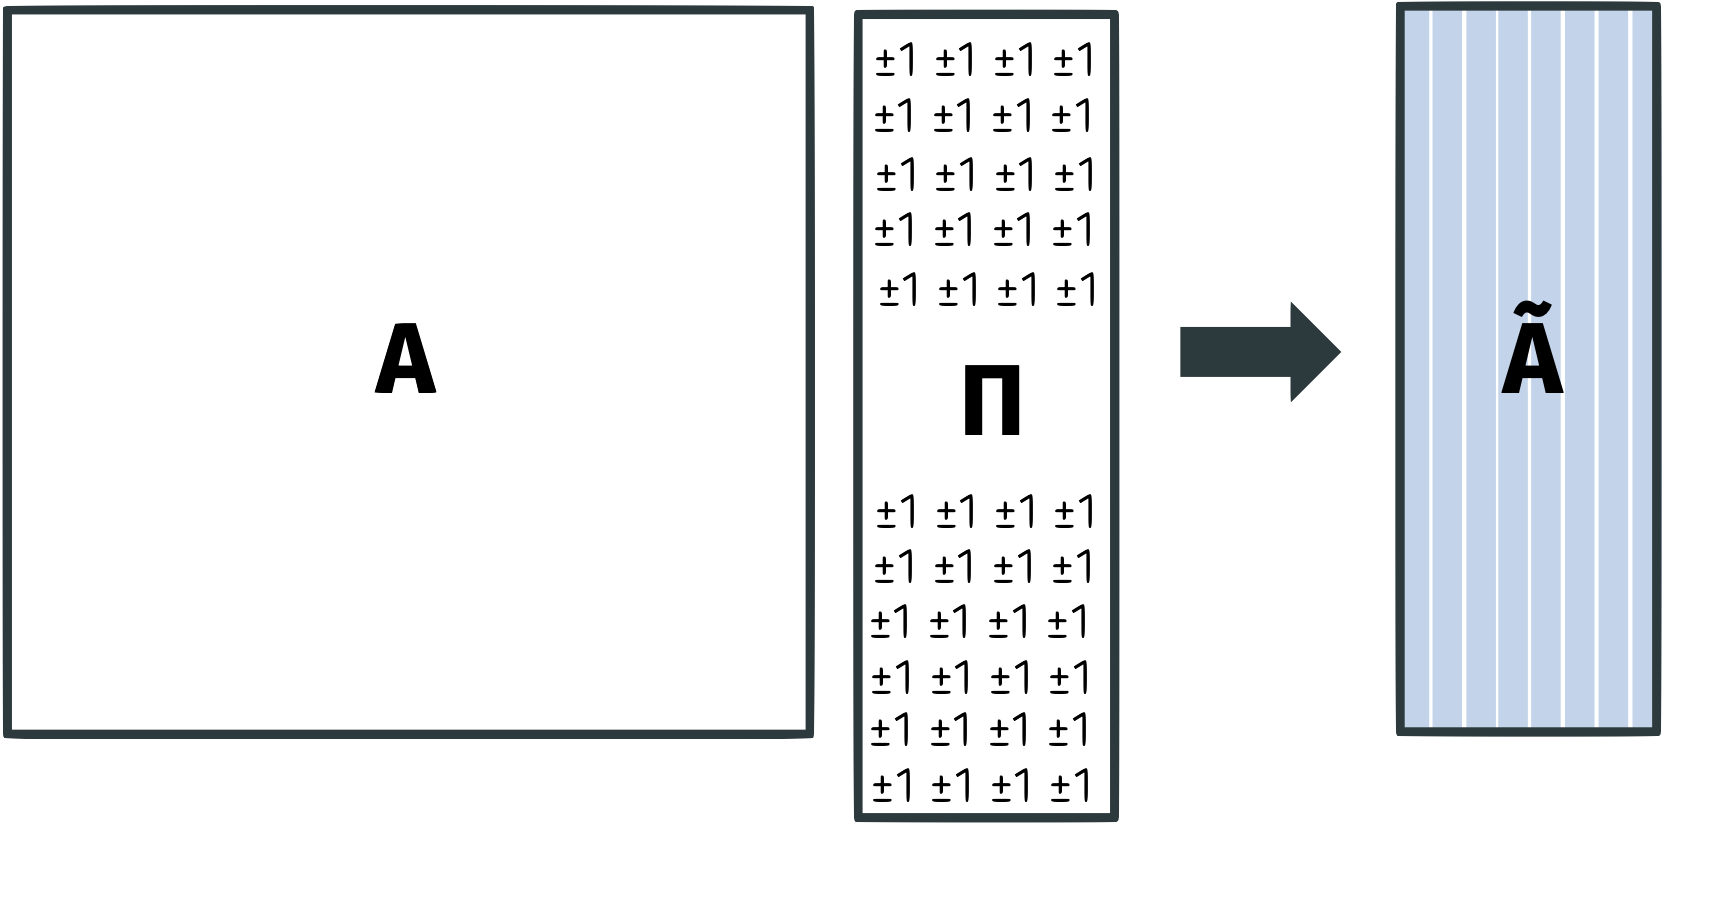
\includegraphics[width=.34\textwidth]{projection_column_reduction1.png}
	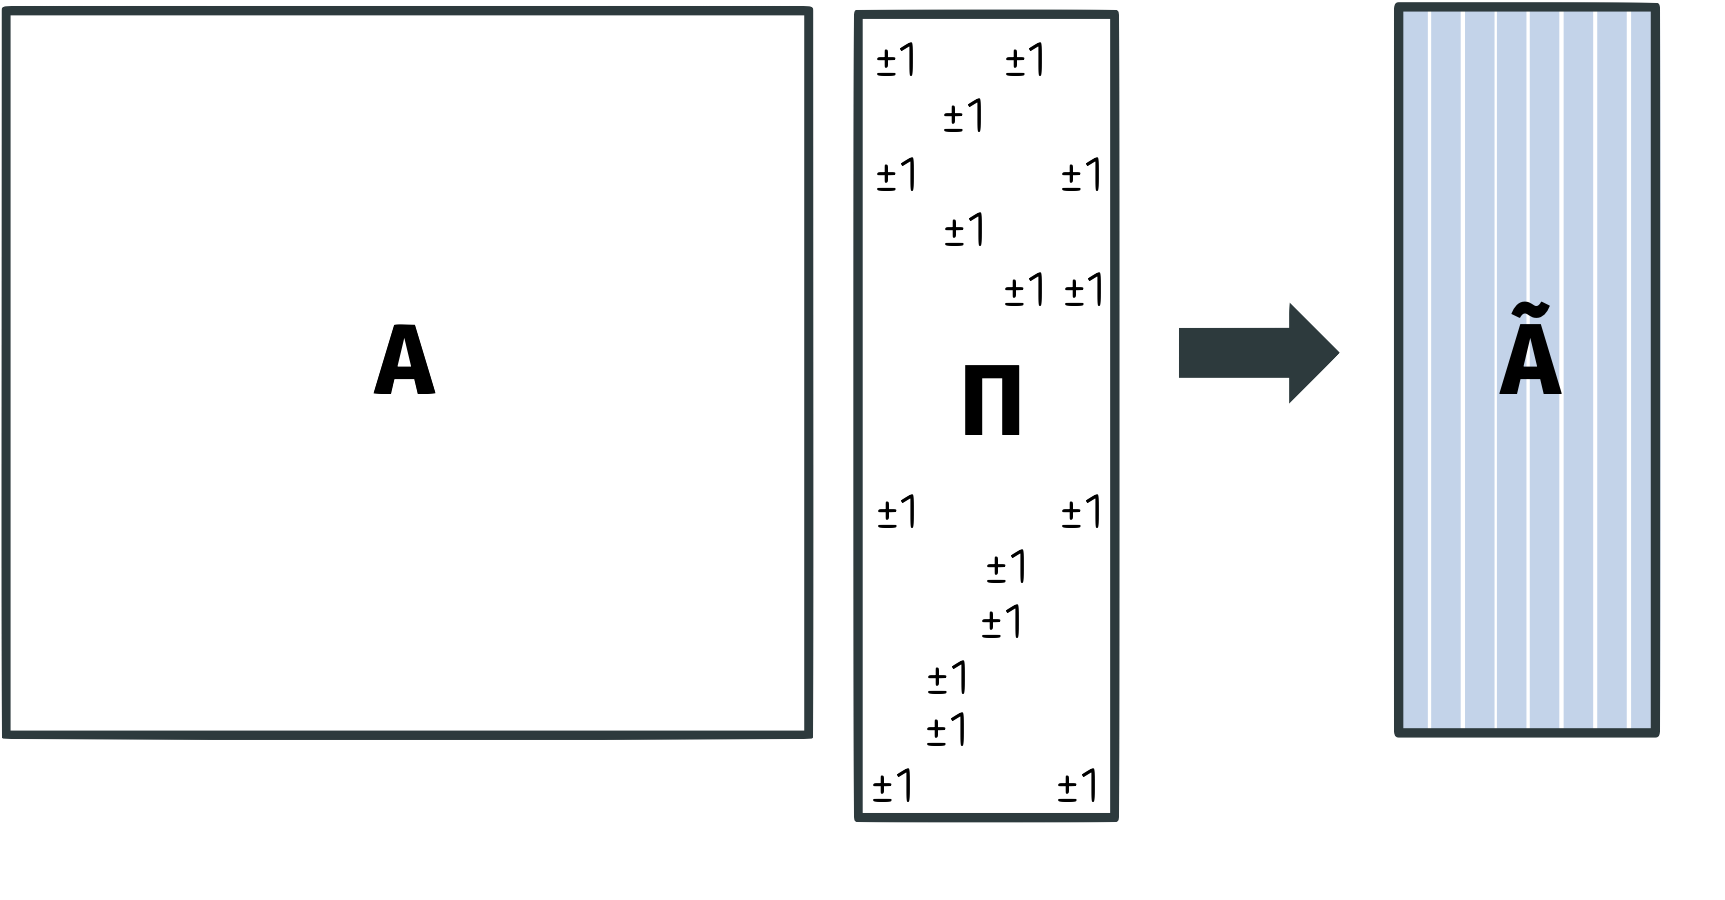
\includegraphics[width=.34\textwidth]{projection_column_reduction2.png}
\end{center}
\end{frame}


\begin{frame}[t]
	\frametitle{sketched regression}
	\textbf{Randomized approximate regression using a Johnson-Lindenstrauss Matrix:}
	\begin{center}
		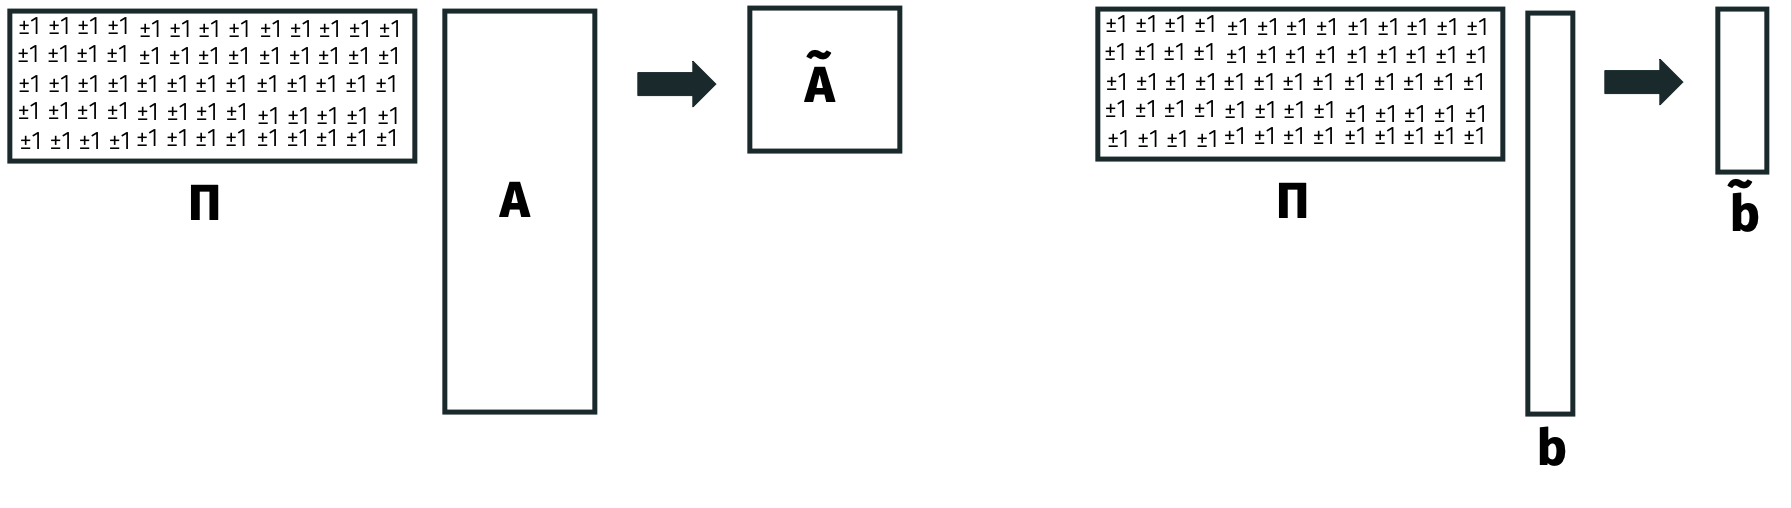
\includegraphics[width=.8\textwidth]{jlRegression.png}
	\end{center}
\vspace{-1em}
	\textbf{Input}: $\bv{A} \in \R^{n\times d}$, $\bv{b} \in \R^{n}$. 
	
	\textbf{Algorithm}: Let $\tilde{\bv{x}}^* = \argmin_{\bv{x}} \|\bs{\Pi}\bv{A}\bv{x} - \bs{\Pi}\bv{b}\|_2^2$.
	
	\textbf{Goal}: Want $\|\bv{A}\tilde{\bv{x}}^* - \bv{b}\|_2^2 \leq (1+\epsilon) \min_{\bv{x}} \|\bv{A}\bv{x} - \bv{b}\|_2^2$
\end{frame}

\begin{frame}[t]
	\frametitle{target result}
	\begin{theorem}[Randomized Linear Regression]
		Let $\bs{\Pi}$ be a properly scaled JL matrix (random Gaussian, sign, sparse random, etc.) with $m = \tilde{O}\left(\frac{d}{\epsilon^2}\right)$ rows. Then with probability $(1-\delta)$, for any $\bv{A}\in \R^{n\times d}$ and $\bv{b}\in \R^n$,
		\begin{align*}
		\|\bv{A}\tilde{\bv{x}}^* - \bv{b}\|_2^2 \leq (1+\epsilon) \min_{\bv{x}} \|\bv{A}\bv{x} - \bv{b}\|_2^2
		\end{align*}
		where $\tilde{\bv{x}}^* = \argmin_{\bv{x}} \|\bs{\Pi}\bv{A}\bv{x} - \bs{\Pi}\bv{b}\|_2^2$.
	\end{theorem}
\end{frame}

\begin{frame}
	\frametitle{subspace embeddings reworded}
	\begin{theorem}[Subspace Embedding]
		Let $\bv{A} \in \R^{n\times d}$ be a matrix. If $\bs{\Pi}\in \R^{m\times n}$ is chosen from any distribution $\mathcal{D}$ satisfying the Distributional JL Lemma, then with probability $1-\delta$,
		\begin{align*}
			(1-\epsilon)\|\bv{A}\bv{x}\|_2^2 \leq \|\bs{\Pi} \bv{A} \bv{x}\|_2^2 \leq	(1+\epsilon)\|\bv{A}\bv{x}\|_2^2
		\end{align*}
		for \emph{all} $\bv{x} \in \R^d$, as long as  $m = {O}\left(\frac{d + \log(1/\delta)}{\epsilon^2}\right)$.
	\end{theorem}
Implies regression result, and more. 

\textbf{Example:} The any singular value $\tilde{\sigma}_i$ of $\bs{\Pi}\bv{A}$ is a $(1\pm \epsilon)$ approximation to the true singular value ${\sigma}_i$ of  $\bv{B}$. 
\end{frame}

\begin{frame}
	\frametitle{subsampling methods}
	\begin{center}
		\textbf{Recurring research interest:} Replace random projection methods with \emph{random sampling methods}. Prove that for essentially all problems of interest, can obtain same asymptotic runtimes. 
		
		\vspace{.5em}
		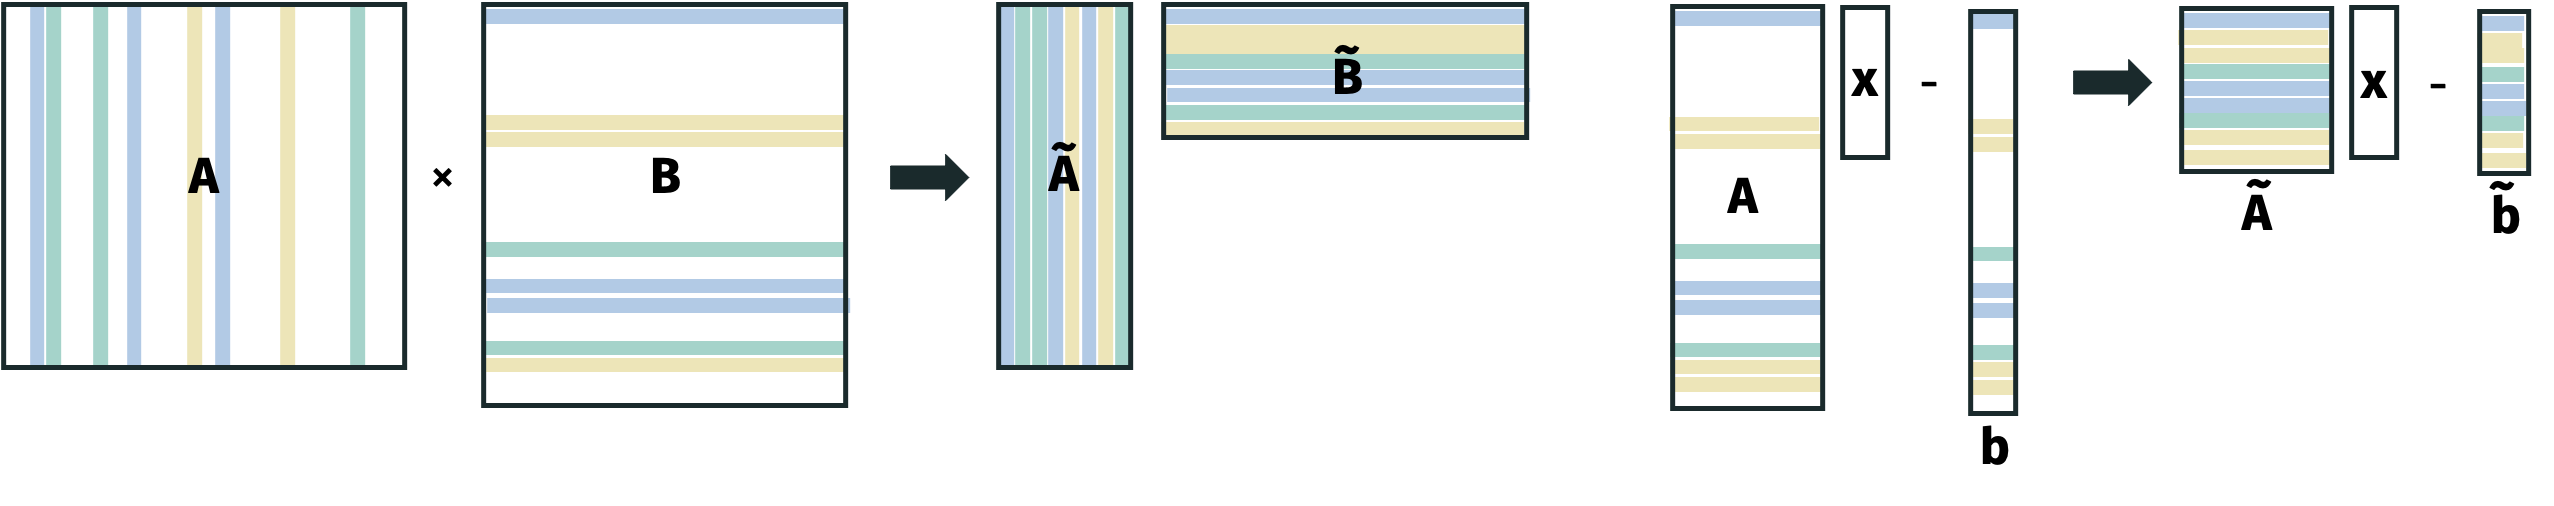
\includegraphics[width=\textwidth]{subsampling_high_level.png}
		
		Sampling has the added benefit of \emph{preserving matrix sparsity or structure}, and can be applied in a \emph{wider variety of settings} where random projections are too expensive.
	\end{center}
\end{frame}


\begin{frame}
	\frametitle{subsampling methods}
	\textbf{First goal:} Can we use sampling to obtain subspace embeddings? I.e. for a given $\bv{A}$ find $\tilde{\bv{A}}$ whose rows are a (weighted) subset of rows in $\bv{A}$ and:
	\begin{align*}
	(1-\epsilon)\|\bv{A}\bv{x}\|_2^2 \leq \|\tilde{\bv{A}}\bv{x}\|_2^2 \leq (1+\epsilon)\|\bv{A}\bv{x}\|_2^2.
	\end{align*}
	\begin{center}
	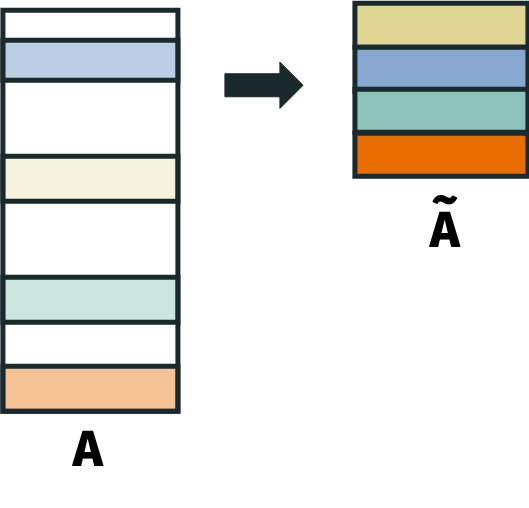
\includegraphics[width=.4\textwidth]{subsampleA.png}
	\end{center}
	
	
\end{frame}

\begin{frame}
	\frametitle{example where structure matters}
	Let $\bv{B}$ be the edge-vertex incidence matrix of a graph $G$ with vertex set $V$, $|V| = d$. Recall that $\bv{B}^T\bv{B} = \bv{L}$.
	\begin{center}
		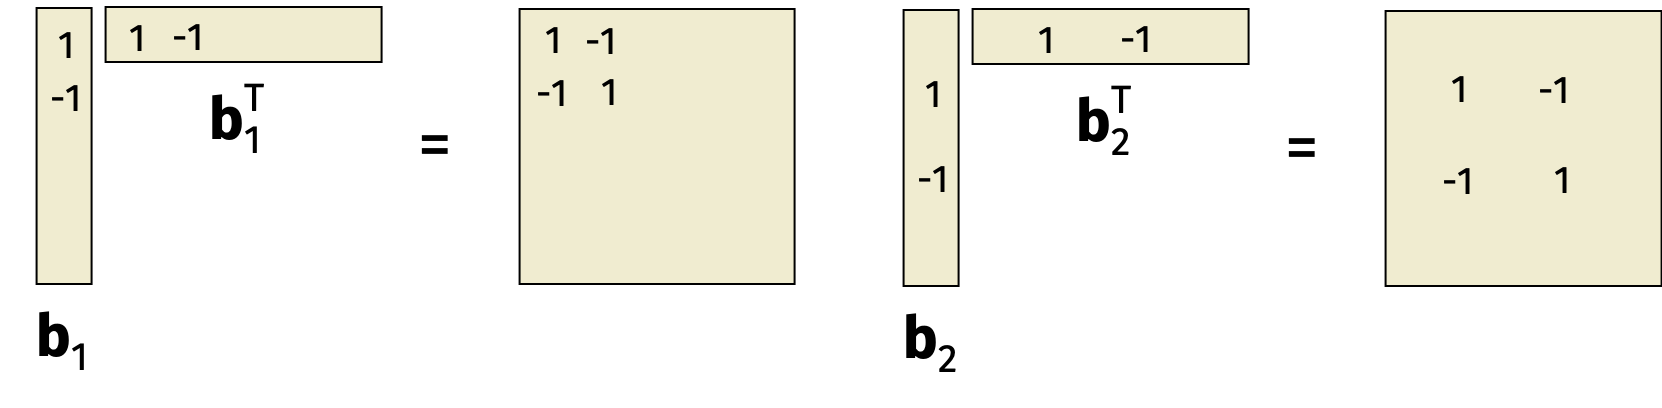
\includegraphics[width=\textwidth]{edge_vertex.png}
	\end{center}
\vspace{-1em}

Recall that if $\bv{x}\in \{-1,1\}^n$ is the \emph{cut indicator vector} for a cut $S$ in the graph, then $\frac{1}{4}\|\bv{B}\bv{x}\|_2^2 = \cut(S,V\setminus S)$.	
\end{frame}

\begin{frame}
	\frametitle{linear algebraic view of cuts}
	\begin{align*}
		\bv{x} = [1,1,1,-1,1,-1,-1,-1]
	\end{align*}
	\begin{center}
		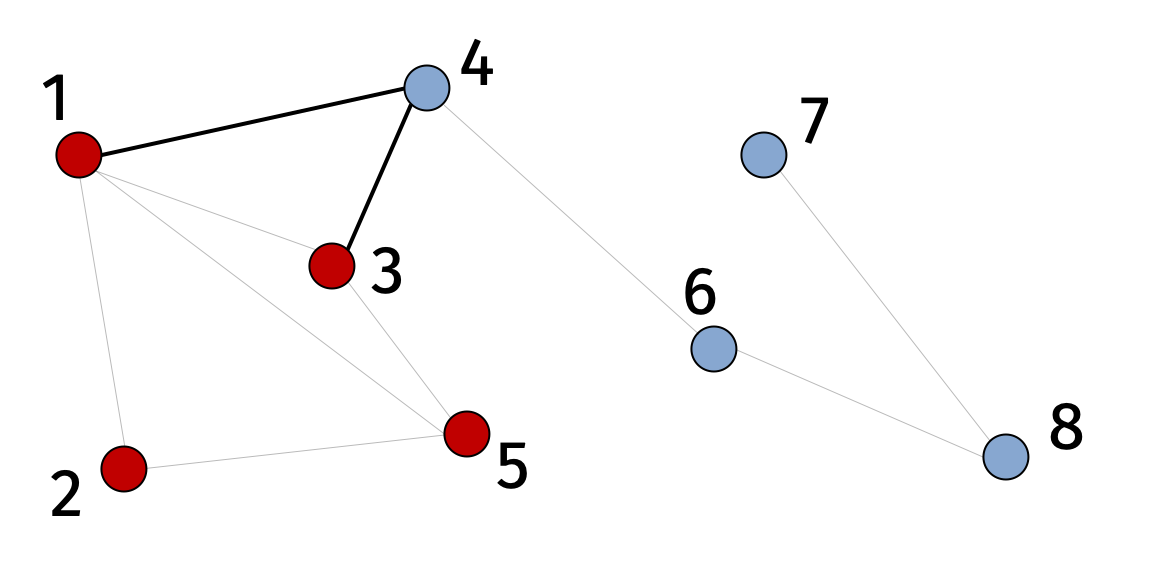
\includegraphics[width=.8\textwidth]{cut_example.png}
	\end{center}
	\vspace{-1em}
	$\bv{x}\in \{-1,1\}^d$ is the \emph{cut indicator vector} for a cut $S$ in the graph, then $\frac{1}{4}\|\bv{B}\bv{x}\|_2^2 = \cut(S,V\setminus S)$	
\end{frame}

\begin{frame}
	\frametitle{weighted cuts}
	Extends to weighted graphs, as long as square root of weights is included in $\bv{B}$. Still have the $\bv{B}^T\bv{B} = \bv{L}$.
	\begin{center}
		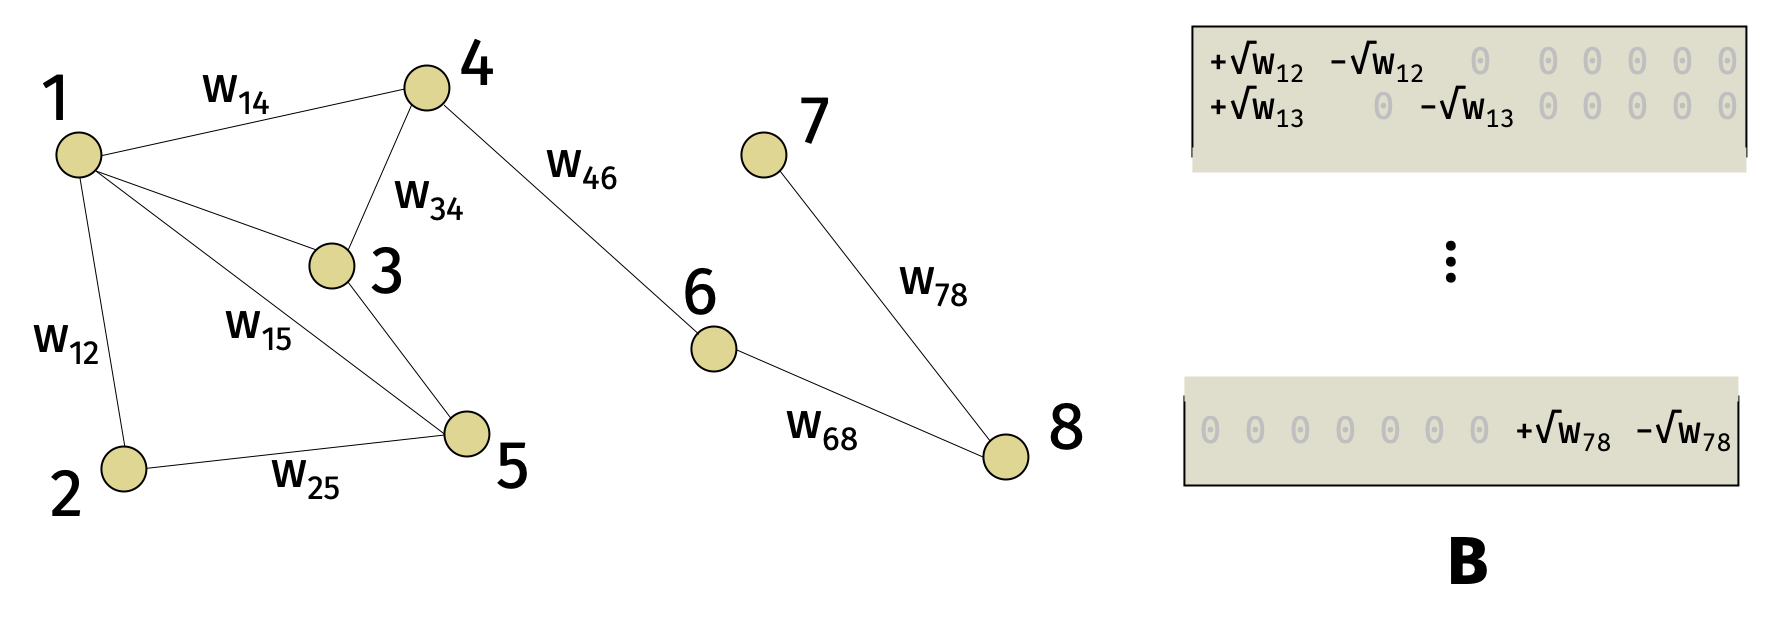
\includegraphics[width=\textwidth]{weighted_edge_vertex.png}
	\end{center}
	\vspace{-1em}
	
	And still have that if $\bv{x}\in \{-1,1\}^d$ is the \emph{cut indicator vector} for a cut $S$ in the graph, then $\frac{1}{4}\|\bv{B}\bv{x}\|_2^2 = \cut(S,V\setminus S)$.	
\end{frame}

\begin{frame}
	\frametitle{spectral sparsification}
	\textbf{Goal:} Approximate $\bv{B}$ by a weighted subsample. I.e. by $\tilde{\bv{B}}$ with $m \ll |E|$ rows, each of which is a scaled copy of a row from $\bv{B}$. 
	\begin{center}
		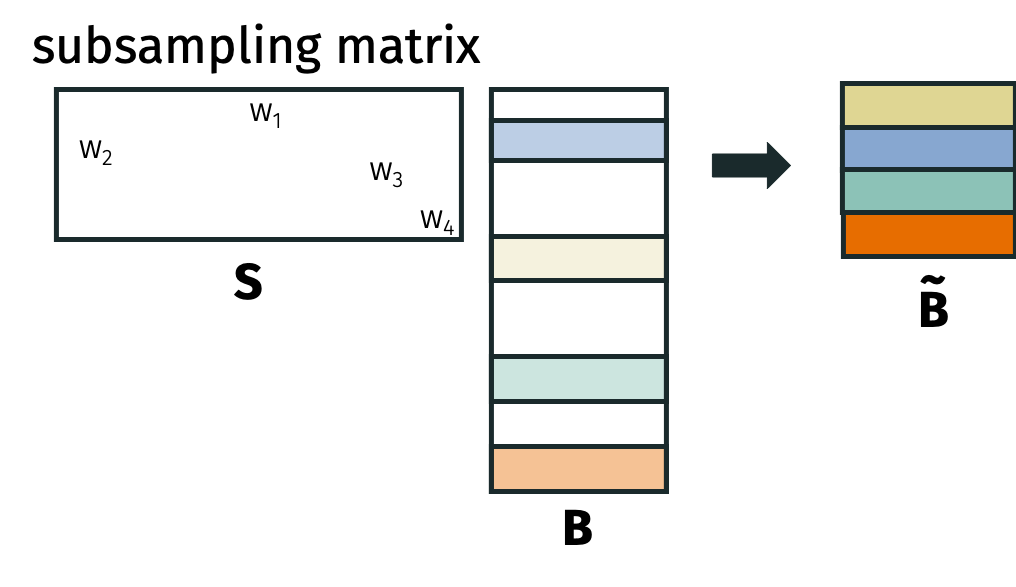
\includegraphics[width=.6\textwidth]{subsampled_b.png}
	\end{center}
\textbf{Natural goal:} $\tilde{\bv{B}}$ is a subspace embedding for $\bv{B}$. In other words, $\tilde{\bv{B}}$ has $\approx O(d)$ rows and for all $\bv{x}$,
\begin{align*}
	(1-\epsilon)\|\bv{B}\bv{x}\|_2^2 \leq \|\tilde{\bv{B}}\bv{x}\|_2^2 \leq (1+\epsilon)\|\bv{B}\bv{x}\|_2^2.
\end{align*} 
\end{frame}

\begin{frame}
	\frametitle{history spectral sparsification}
	$\tilde{\bv{B}}$ is itself an edge-vertex incidence matrix for some 
\emph{sparser} graph $\tilde{G}$, which preserves many properties about $G$!  $\tilde{G}$ is called a \emph{spectral sparsifier} for $G$.
\vspace{-1em}

	\begin{center}
		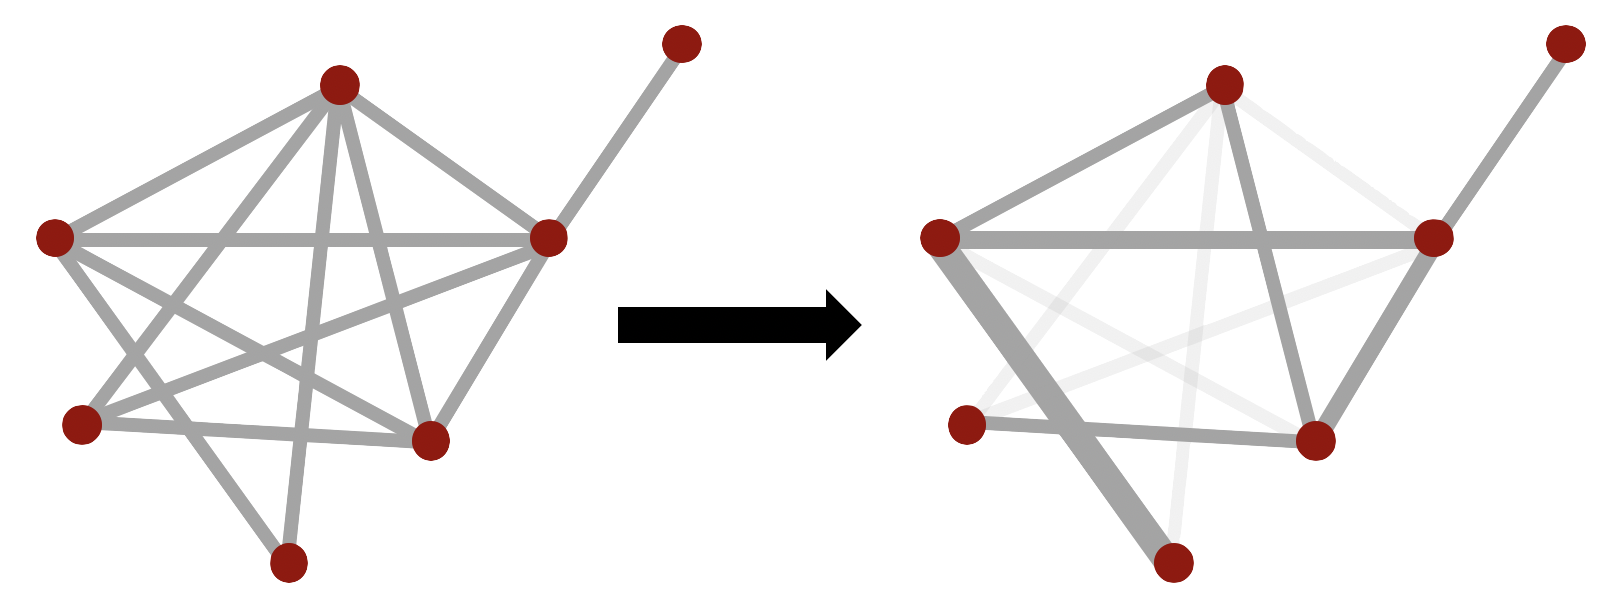
\includegraphics[width=.6\textwidth]{sparsifier.png}
	\end{center}

\vspace{-1em}
  For example, we have that for any set $S$, 
	\begin{align*}
		(1-\epsilon)\cut_{{G}}(S,V\setminus S) \leq \cut_{\tilde{G}}(S,V\setminus S) \leq (1+\epsilon)\cut_{{G}}(S,V\setminus S).
	\end{align*}
So $\tilde{G}$ can be used in place of $G$ in solving e.g. max/min cut problems, balanced cut problems, etc. 

\vspace{-1em}
\begin{center}
	\alert{In contrast $\bs{\Pi} \bv{B}$ would look nothing like an edge-vertex incidence matrix if $\bs{\Pi}$ is a JL matrix. }
\end{center}
\end{frame}


\begin{frame}[t]
	\frametitle{history of spectral sparsification}
	Spectral sparsifiers were introduced in 2004 by Spielman and Teng in an influential paper on faster algorithms for solving Laplacian linear systems. 
	\begin{itemize}
		\item Generalize the cut sparsifiers of Benczur, Karger `96. 
		\item Further developed in work by Spielman, Srivastava + Batson, `08.
		\item Have had huge influence in algorithms, and other areas of mathematics -- this line of work lead to the 2013 resolution of the Kadison-Singer problem in functional analysis by Marcus, Spielman, Srivastava. 
	\end{itemize}
	\alert{\textbf{This class}: Learn about an important random sampling algorithm for constructing spectral sparsifiers, and subspace embeddings for matrices more generally.}
\end{frame}

\begin{frame}[t]
	\frametitle{natural first attempt}
	\textbf{Goal:} Find $\tilde{\bv{A}}$ such that $\|\tilde{\bv{A}}\bv{x}\|_2^2 = (1\pm \epsilon)\|{\bv{A}}\bv{x}\|_2^2$ for all $\bv{x}$. 
	
	\textbf{Possible Approach:} Construct ${\tilde{\bv{A}}}$ by \emph{uniformly sampling} rows from $\bv{A}$. 
	
	\vspace{-2.5em}
	\begin{center}
		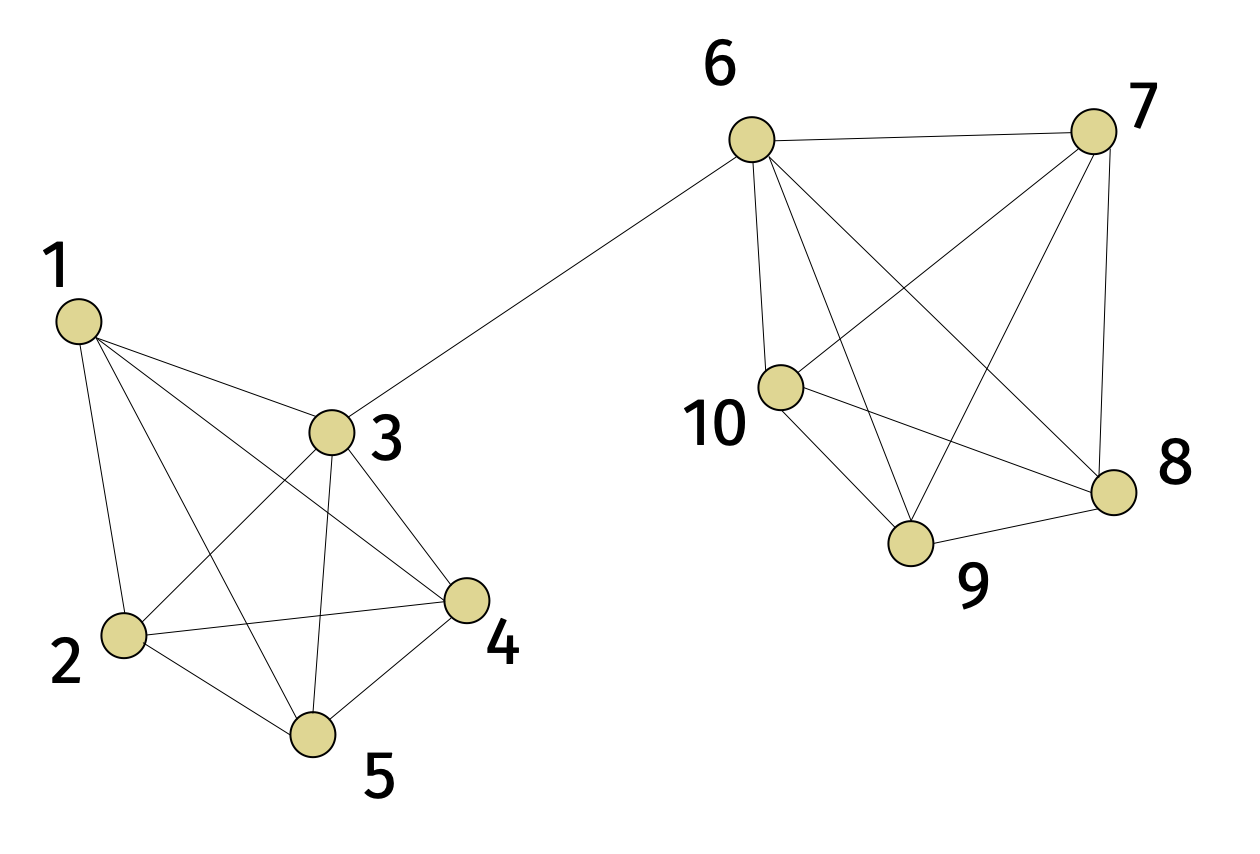
\includegraphics[width=.8\textwidth]{barbell.png}
		
		\vspace{-1.5em}
		Can check that this approach fails even for the special case of a graph vertex-edge incidence matrix. 
	\end{center}	
\end{frame}

\begin{frame}[t]
	\frametitle{importance sampling framework}
	\textbf{Key idea:} \emph{Importance sampling}. Select some rows with higher probability. 
	
	Suppose $\bv{A}$ has $n$ rows $\bv{a}_1\ldots, \bv{a}_n$. Let $p_1, \ldots, p_n \in [0,1]$ be sampling probabilities. Construct $\tilde{\bv{A}}$ as follows:
	\begin{itemize}
		\item For $i = 1,\ldots, n$
		\begin{itemize}
			\item Select $\bv{a}_i$ with probability $p_i$. 
			\item If $\bv{a}_i$ is selected, add the scaled row $\frac{1}{\sqrt{p_i}} \bv{a}_i$ to $\tilde{A}$. 
		\end{itemize}
	\end{itemize}
Remember, ultimately want that $\|\tilde{\bv{A}}\bv{x}\|_2^2 = (1\pm \epsilon)\|{\bv{A}}\bv{x}\|_2^2$ for all $\bv{x}$. 

	\textbf{Claim 1:} $\E[\|\tilde{\bv{A}}\bv{x}\|_2^2] = \|{\bv{A}}\bv{x}\|_2^2$. 
	\vspace{2em}
	
	
	\textbf{Claim 2:} Expected number of rows in $\tilde{\bv{A}}$ is $\sum_{i=1}^n p_i$. 
\end{frame}

\begin{frame}[t]
	\frametitle{lecture outline}
	\begin{center}
		\alert{\textbf{How should we choose the probabilities $p_1, \ldots, p_n$?}}
	\end{center}
	\begin{enumerate}
		\item Introduce the idea of row \textbf{leverage scores}. 
		\item Motivate why these scores make for good sampling probabilities. 
		\item Prove (at least mostly) that sampling with probabilities proportional to these scores yields a subspace embedding (or a spectral sparsifier) with a near optimal number of rows.
	\end{enumerate}
\end{frame}

\begin{frame}[t]
	\frametitle{main result}
	Let $\bv{a}_1, \ldots, \bv{a}_n$ be $\bv{A}$'s rows. We define the \alert{\textbf{statistical leverage score}} $\tau_i$ of row $\bv{a}_i$ as:
	\begin{align*}
		\tau_i = \bv{a}_i^T(\bv{A}^T\bv{A})^{-1}\bv{a}_i.
	\end{align*}	
We will show that $\tau_i$ is a natural \emph{importance measure} for each row in $\bv{A}$.

We have that $\tau_i \in [0,1]$ and $\sum_{i=1}^n \tau_i = d$ if $\bv{A}$ has $d$ columns. 


\end{frame}

\begin{frame}[t]
	\frametitle{main result}
	For $i = 1, \ldots, n$,
	\begin{align*}
		\tau_i = \bv{a}_i^T(\bv{A}^T\bv{A})^{-1}\bv{a}_i.
	\end{align*}	
	\begin{theorem}[Subspace Embedding from Subsampling]
		For each $i$, and fixed constant $c$, let $p_i = \min\left(1,\frac{c\log d}{\epsilon^2}\cdot \tau_i\right)$.
		Let ${\tilde{\bv{A}}}$ have rows sampled from $\bv{A}$ with probabilities $p_1, \ldots, p_n$. With probability $9/10$, 
		\begin{align*}
			(1-\epsilon)\|\bv{A}\bv{x}\|_2^2 \leq \|\tilde{\bv{A}} \bv{x}\|_2^2 \leq	(1+\epsilon)\|\bv{A}\bv{x}\|_2^2,
		\end{align*}
		and ${\tilde{\bv{A}}}$ has $O(d\log d/\epsilon^2)$ rows in expectation. 
	\end{theorem}
\end{frame}


\begin{frame}[t]
	\frametitle{vector sampling}
	\begin{center}
		How should we choose the probabilities $p_1, \ldots, p_n$?
	\end{center}
	As usual, consider a single vector $\bv{x}$ and understand how to sample to preserve norm of $\bv{y} = \bv{A}\bv{x}$:
	\begin{align*}
		\|\tilde{\bv{A}}\bv{x}\|_2^2 = \|\bv{S}{\bv{A}}\bv{x}\|_2^2 = \|\bv{S}\bv{y}\|_2^2 \approx \|\bv{y}\|_2^2 = \|\bv{Ax}\|_2^2. 
	\end{align*}
	Then we can union bound over an $\epsilon$-net to extend to all $\bv{x}$. 
\end{frame}

\begin{frame}[t]
	\frametitle{vector sampling}
	As discussed a few lectures ago, uniform sampling only works well if $\bv{y} = \bv{A}\bv{x}$ is ``flat''. 
	\vspace{-.5em}
	\begin{center}
		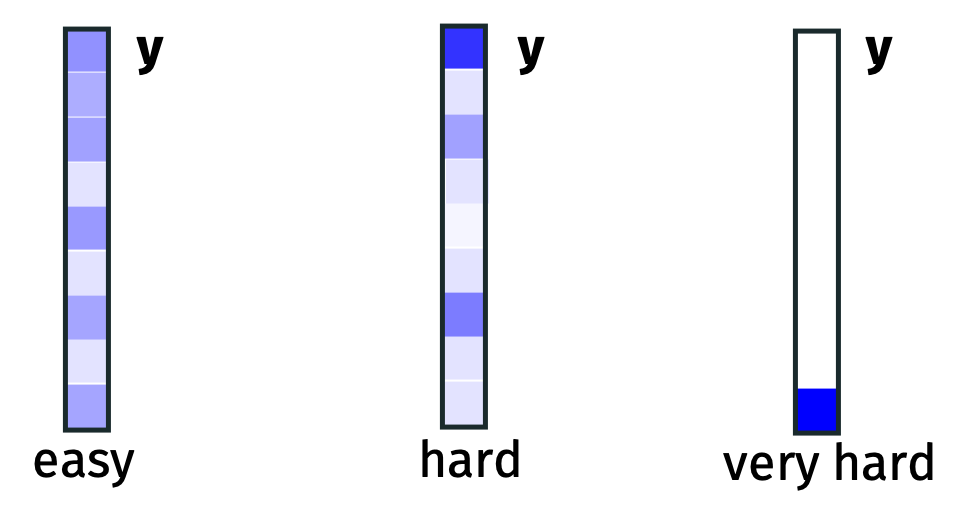
\includegraphics[width=.6\textwidth]{uniform_hard.png}
	\end{center}
	\vspace{-.5em}
		
	Instead consider sampling with probabilities at least \emph{proportional to the magnitude of $\bv{y}$'s entries}:
	\begin{align*}
		p_i > c\cdot \frac{y_i^2}{\|y\|_2^2} \text{ for constant $c$ to be determined.}
	\end{align*}
\end{frame}

\begin{frame}[t]
	\frametitle{variance analysis}	
	Let $\tilde{\bv{y}}$ be the subsampled $\bv{y}$. Recall that, when sampling with probabilities $p_1, \ldots, p_n$, for $i = 1,\ldots, n$ we add $y_i$ to $\tilde{\bv{y}}$ with probability $p_i$ and reweight by $\frac{1}{\sqrt{p_i}}$. 
	
	$\|\tilde{\bv{y}}\|_2^2 = $
	
	$\sigma^2 = \Var[\|\tilde{\bv{y}}\|_2^2] = $
\end{frame}	

\begin{frame}[t]
	\frametitle{variance analysis}	
	Recall Chebyshev's Inequality:
	\begin{align*}
		\Pr[\left|\|\tilde{\bv{y}}\|_2^2 - \|\bv{y}\|_2^2\right| \leq \frac{1}{\sqrt{\delta}}\cdot \sigma] \leq \delta
	\end{align*}
	We want error $\left|\|\tilde{\bv{y}}\|_2^2 - \|\bv{y}\|_2^2\right| \leq \epsilon \|\bv{y}\|_2^2$. 
	
	Need set $c = \frac{1}{\delta\epsilon^2}$.\footnote{\footnotesize Using the right Bernstein bound we can improve to $c  = O(\log(1/\delta)/\epsilon^2)$.} 
	
	If we \emph{knew} $y_1, \ldots, y_n$, the number of samples we take in expectation is:
	\begin{align*}
		\sum_{i=1}^n p_i = \sum_{i=1}^n c\cdot \frac{y_i^2}{\|y_i\|_2^2} = \frac{1}{\delta\epsilon^2}. 
	\end{align*}
\end{frame}

\begin{frame}[t]
	\frametitle{maximization characterization}	
	But we of course don't know $y_1, \ldots, y_n$, and even so these values aren't fixed. We wanted to prove a bound for $\bv{y} = \bv{A}\bv{x}$ for \emph{any} $\bv{x}$. 
	
	\textbf{Idea behind leverage scores:} Sample row $i$ from $\bv{A}$ using the \emph{worst case} (largest necessary) sampling probability:
	\begin{align*}
		\tau_i &= \max_{\bv{x}} \frac{y_i^2}{\|\bv{y}\|_2^2} &&\text{where} & \bv{y} = \bv{A}\bv{x}. 
	\end{align*}
If we sample with probability $p_i = \frac{1}{\epsilon^2}\cdot \tau_i$, then we will be sampling by at least $\frac{1}{\epsilon^2}\cdot\frac{y_i^2}{\|y\|_2^2}$, \emph{no matter what $\bv{y}$ is}. 

Two major concerns: 1) How to compute $\tau_1, \ldots, \tau_n$, and 2) the number of samples we take will be roughly $\sum_{i=1}^n \tau_i$. How do we bound this?
\end{frame}	


\begin{frame}[t]
	\frametitle{maximization characterization}
	\begin{align*}
		\tau_i &= \max_{\bv{x}} \frac{y_i^2}{\|\bv{y}\|_2^2} &&\text{where} & \bv{y} = \bv{A}\bv{x}. 
	\end{align*}
	\vspace{9em}
	
	\textbf{Recall Cauchy-Schwarz inequality}: $(\bv{w}^T\bv{z})^2 \leq \bv{w}^T\bv{w}\cdot \bv{z}^T\bv{z}$
\end{frame}

\begin{frame}[t]
	\frametitle{equivalent minimization characterization}
	\begin{align*}
		\tau_i &= \min_{\bv{z} \text{ such that } \bv{A}^T\bv{z} = \bv{a}_i} \|\bv{z}\|_2^2. 
	\end{align*}
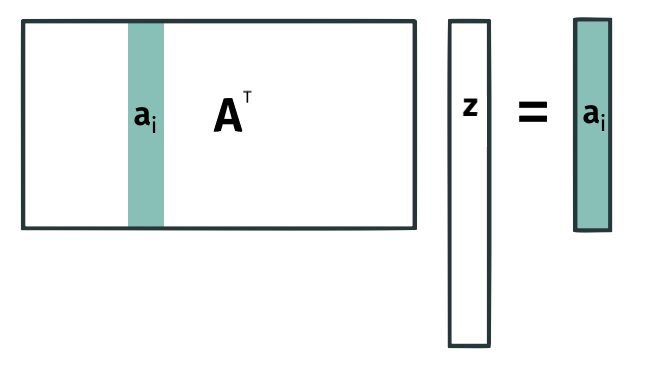
\includegraphics[width=.6\textwidth]{minchar_1.png}
\end{frame}

\begin{frame}[t]
	\frametitle{equivalent minimization characterization}
	\begin{align*}
		\tau_i &= \min_{\bv{z} \text{ such that } \bv{A}^T\bv{z} = \bv{a}_i} \|\bv{z}\|_2^2. 
	\end{align*}
	\begin{columns}
		\begin{column}{.5\textwidth}
			\centering
			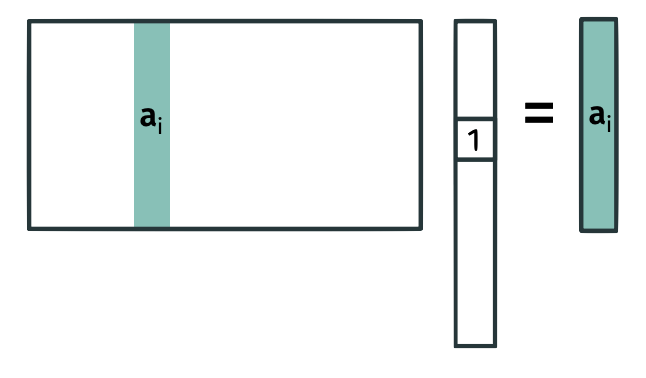
\includegraphics[width=\textwidth]{minchar_2.png}
		\end{column}
		\begin{column}{.5\textwidth}
						\centering
			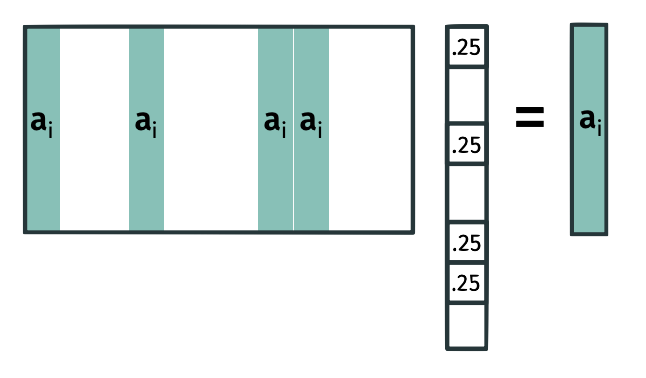
\includegraphics[width=\textwidth]{minchar_3.png}
		\end{column}
	\end{columns}
\begin{center}
	\textbf{\alert{Gives clearer picture of leverage score $\tau_i$ as a measure of ``uniqueness'' for row $\bv{a}_i$.}}
\end{center}
\end{frame}

\begin{frame}[t]
	\frametitle{leverage score sampling}
	\textbf{Leverage score sampling:}
	\begin{itemize}
		\item For $i = 1, \ldots, n$, 
		\begin{itemize}
			\item Compute $\tau_i = \bv{a}_i^T(\bv{A}^T\bv{A})^{-1}\bv{a}_i$. 
			\item Set $p_i = \frac{c\log(1/\delta)}{\epsilon^2}\cdot \tau_i$.
			\item Add row $\bv{a}_i$ to $\tilde{\bv{A}}$ with probability $p_i$ and reweight by $\frac{1}{\sqrt{p_i}}$.  			
		\end{itemize}
	\end{itemize}
	For any fixed $\bv{x}$, we will have that $(1-\epsilon) \|{\bv{A}}\bv{x}\|_2^2\leq \|\tilde{\bv{A}}\bv{x}\|_2^2 \leq (1+\epsilon) \|{\bv{A}}\bv{x}\|_2^2$ with probability $(1-\delta)$. 
	
	\begin{center}
	\alert{How many rows do we sample in expectation?}
	\end{center}
\end{frame}

\begin{frame}[t]
	\frametitle{sum of leverage scores}
	\textbf{Claim:} No matter how large $n$ is, $\sum_{i=1}^n \tau_i = d$ a matrix $\bv{A}\in \R^d$. 
	
	
	\vspace{12em}
	\begin{center}
		\alert{``Zero-sum'' law for the importance of matrix rows.}
	\end{center}
\end{frame}

\begin{frame}[t]
	\frametitle{leverage score sampling}
		\textbf{Leverage score sampling:}
	\begin{itemize}
		\item For $i = 1, \ldots, n$, 
		\begin{itemize}
			\item Compute $\tau_i = \bv{a}_i^T(\bv{A}^T\bv{A})^{-1}\bv{a}_i$. 
			\item Set $p_i = \frac{c\log(1/\delta}{\epsilon^2}\cdot \tau_i$.
			\item Add row $\bv{a}_i$ to $\tilde{\bv{A}}$ with probability $p_i$ and reweight by $\frac{1}{\sqrt{p_i}}$.  			
		\end{itemize}
	\end{itemize}
	For any fixed $\bv{x}$, we will have that $(1-\epsilon) \|{\bv{A}}\bv{x}\|_2^2\leq \|\tilde{\bv{A}}\bv{x}\|_2^2 \leq (1+\epsilon) \|{\bv{A}}\bv{x}\|_2^2$ with high probability. 
	
	And since $\sum_{i=1}^n p_i = \frac{c\log(1/\delta}{\epsilon^2}\cdot \sum_{i=1}^n \tau_i$,  $\tilde{\bv{A}}$ contains $O\left(\frac{d\log(1/\delta)}{\epsilon^2}\right)$ rows in expectation.

\begin{center}
	Last step: need to extend to all $\bv{x}$. 	
\end{center}
\end{frame}

\begin{frame}[t]
	\frametitle{main result}
	Naive $\epsilon$-net argument leads to $d^2$ dependence since we need to set $\delta = c^d$. Getting the right $d\log d$ dependence below requires a standard ``matrix Chernoff bound'' (see e.g. Tropp 2015). 
	\begin{theorem}[Subspace Embedding from Subsampling]
		For each $i$, and fixed constant $c$, let $p_i = \min\left(1,\frac{c\log d}{\epsilon^2}\cdot \tau_i\right)$.
		Let ${\tilde{\bv{A}}}$ have rows sampled from $\bv{A}$ with probabilities $p_1, \ldots, p_n$. With probability $9/10$, 
		\begin{align*}
			(1-\epsilon)\|\bv{A}\bv{x}\|_2^2 \leq \|\tilde{\bv{A}} \bv{x}\|_2^2 \leq	(1+\epsilon)\|\bv{A}\bv{x}\|_2^2,
		\end{align*}
		and ${\tilde{\bv{A}}}$ has $O(d\log d/\epsilon^2)$ rows in expectation. 
	\end{theorem}
\end{frame}

\begin{frame}[t]
	\frametitle{spectral sparsification corollary}
	For any graph $G$ with $d$ nodes, there exists a graph $\tilde{G}$ with $O(d\log d/\epsilon^2)$ edges such that, for all $\bv{x}$, $\|\tilde{\bv{B}}\bv{x}\|_2^2 = (1\pm\epsilon)\|{\bv{B}}\bv{x}\|_2^2$. 
	\begin{center}
		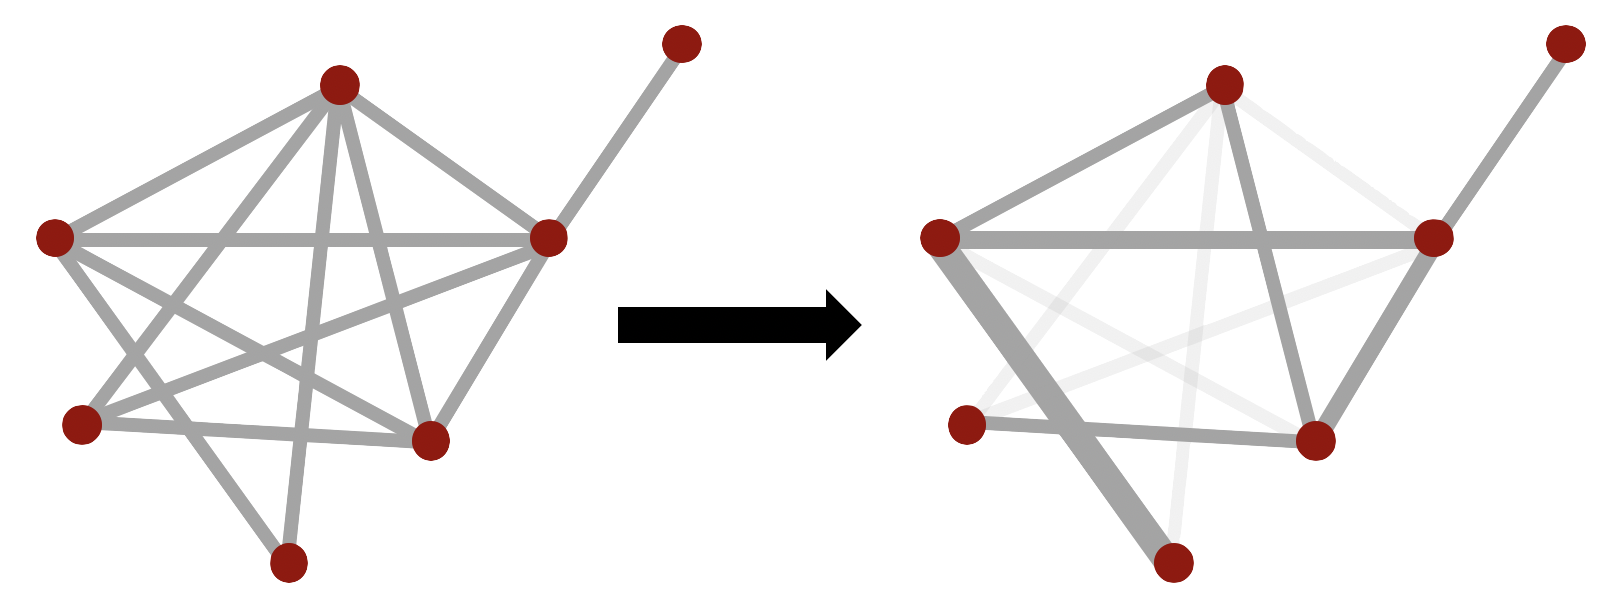
\includegraphics[width=.6\textwidth]{sparsifier.png}
	\end{center}
As a result, the value of any cut in $\tilde{G}$ is within a $(1\pm \epsilon)$ factor of the value in $G$, the Laplacian eigenvalues are with a $(1\pm \epsilon)$ factors, etc. 
\end{frame}

\begin{frame}[t]
	\frametitle{another application: active regression}	
	In many applications, computational costs are second order to \emph{data collection costs.} We have a huge range of possible data points $\bv{a}_1, \ldots, \bv{a}_n$ that we can collect labels/values $b_1,\ldots, b_n$ for. Goal is to learn $\bv{x}$ such that:
	\begin{align*}
		\bv{a}_i^T\bv{x} \approx b_i.
	\end{align*}
Want to do so after observing as few $b_1, \ldots, b_n$ as possible. 
Applications include healthcare, environmental science, etc. 
\begin{center}
	\vspace{-.5em}
	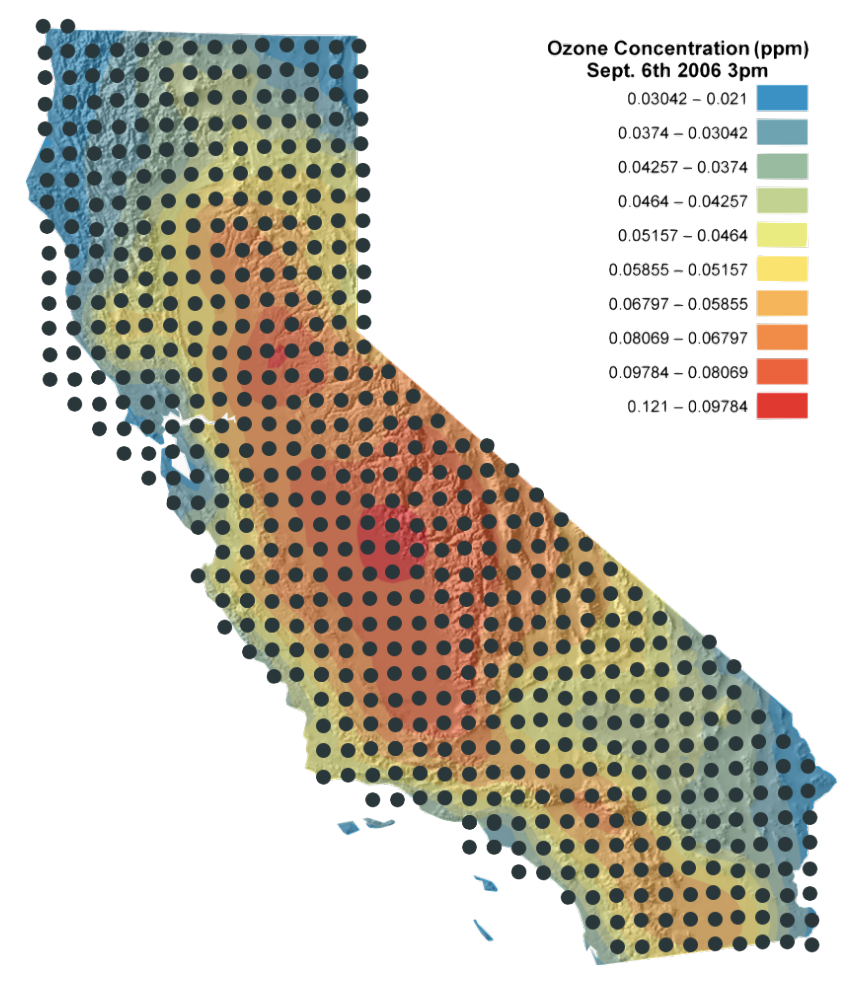
\includegraphics[width=.3\textwidth]{cali.png}
\end{center}
\end{frame}	

\begin{frame}[t]
	\frametitle{another application: active regression}	
\textbf{Can be solved via random sampling} for linear models.
	\begin{center}
		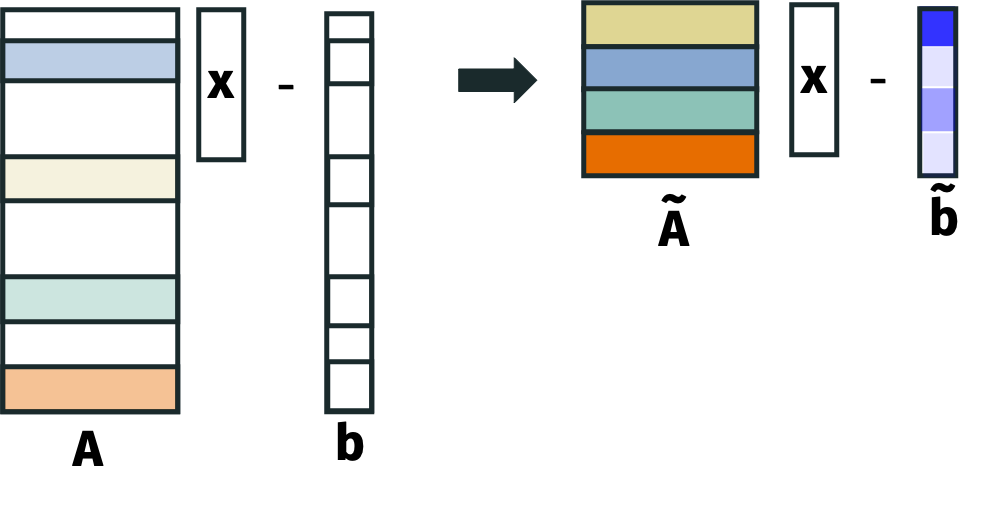
\includegraphics[width=.6\textwidth]{active_regression.png}
	\end{center}
\end{frame}	

\begin{frame}[t]
	\frametitle{another application: active regression}	
	\textbf{Claim:} Let $\tilde{\bv{A}}$ is an $O(1)$-factor subspace embedding for $\bv{A}$ (obtained via leverage score sampling). Then $\tilde{\bv{x}} = \argmin \|\tilde{\bv{A}}\bv{x} - \tilde{\bv{b}}\|_2^2$ satisfies:
	\begin{align*}
		\|\bv{A}\tilde{\bv{x}} - \bv{b}\|_2^2 \leq O(1) \|\bv{A}\bv{x}^* - \bv{b}\|_2^2, 
	\end{align*}
where $\bv{x}^* = \argmin \|{\bv{A}}\bv{x} - \bv{b}\|_2^2$. Computing $\tilde{\bv{x}}$ only requires collecting $O(d\log d)$ labels (independent of $n$). 

\textbf{Lots of applications:}
\begin{itemize}
	\item Robust bandlimited, multiband, and polynomial interpolation [STOC 2019].
	\item Robust active learning for Gaussian process regression [NeurIPS 2020].
\end{itemize}
	
\end{frame}

\begin{frame}[t]
	\frametitle{another application: active regression}	
	\textbf{Claim:} $\tilde{\bv{x}} = \argmin \|\tilde{\bv{A}}\bv{x} - \tilde{\bv{b}}\|_2^2$ satisfies:
	\begin{align*}
		\|\bv{A}\tilde{\bv{x}} - \bv{b}\|_2^2 \leq O(1) \|\bv{A}\bv{x}^* - \bv{b}\|_2^2, 
	\end{align*}
	where $\bv{x}^* = \argmin \|{\bv{A}}\bv{x} - \bv{b}\|_2^2$. Computing $\tilde{\bv{x}}$ only requires collecting $O(d\log d)$ labels (independent of $n$). 
	
	\textbf{Proof:}
	
\end{frame}


\begin{frame}[t]
	\frametitle{some other things i have worked on}
	\textbf{Problem}: Computing leverage scores $\tau_i = \bv{a}_i^T(\bv{A}^T\bv{A})^{-1}\bv{a}_i$ is expensive. 	\vspace{-.5em}

		
		\begin{center}
			\uncover<2->{\only<1-2>{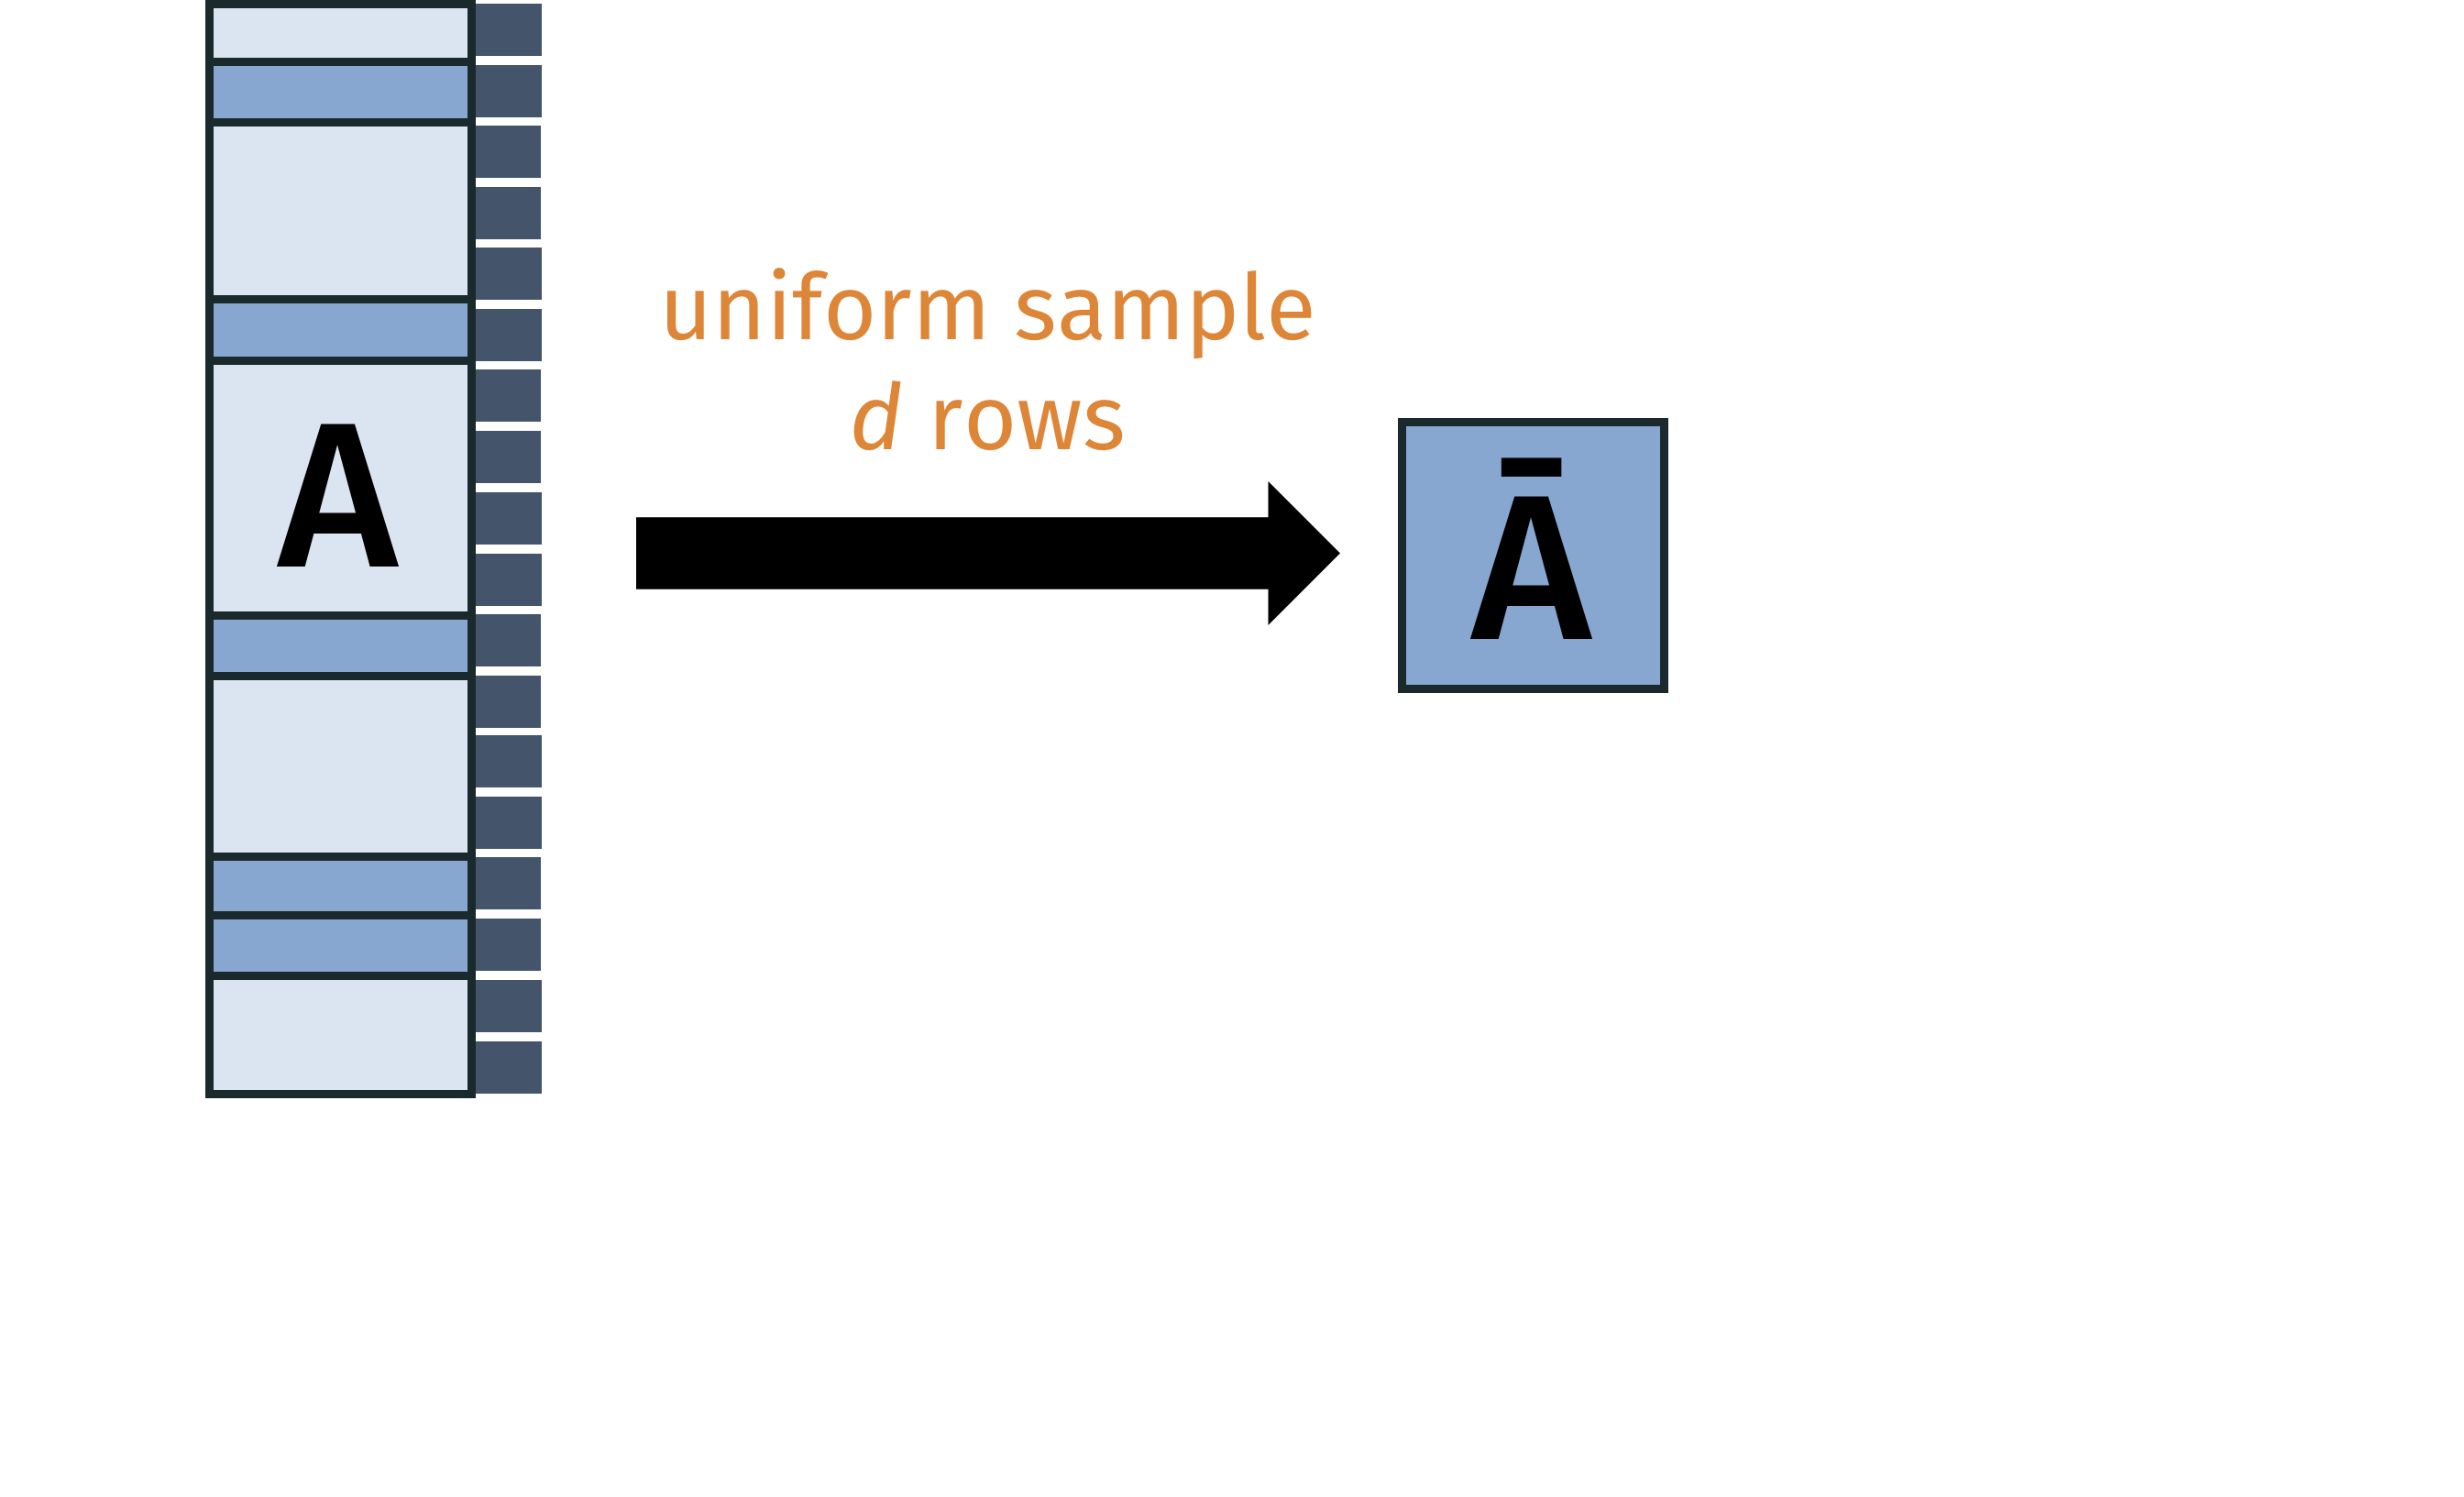
\includegraphics[width=.7\textwidth]{algo1.png}}
				\only<3>{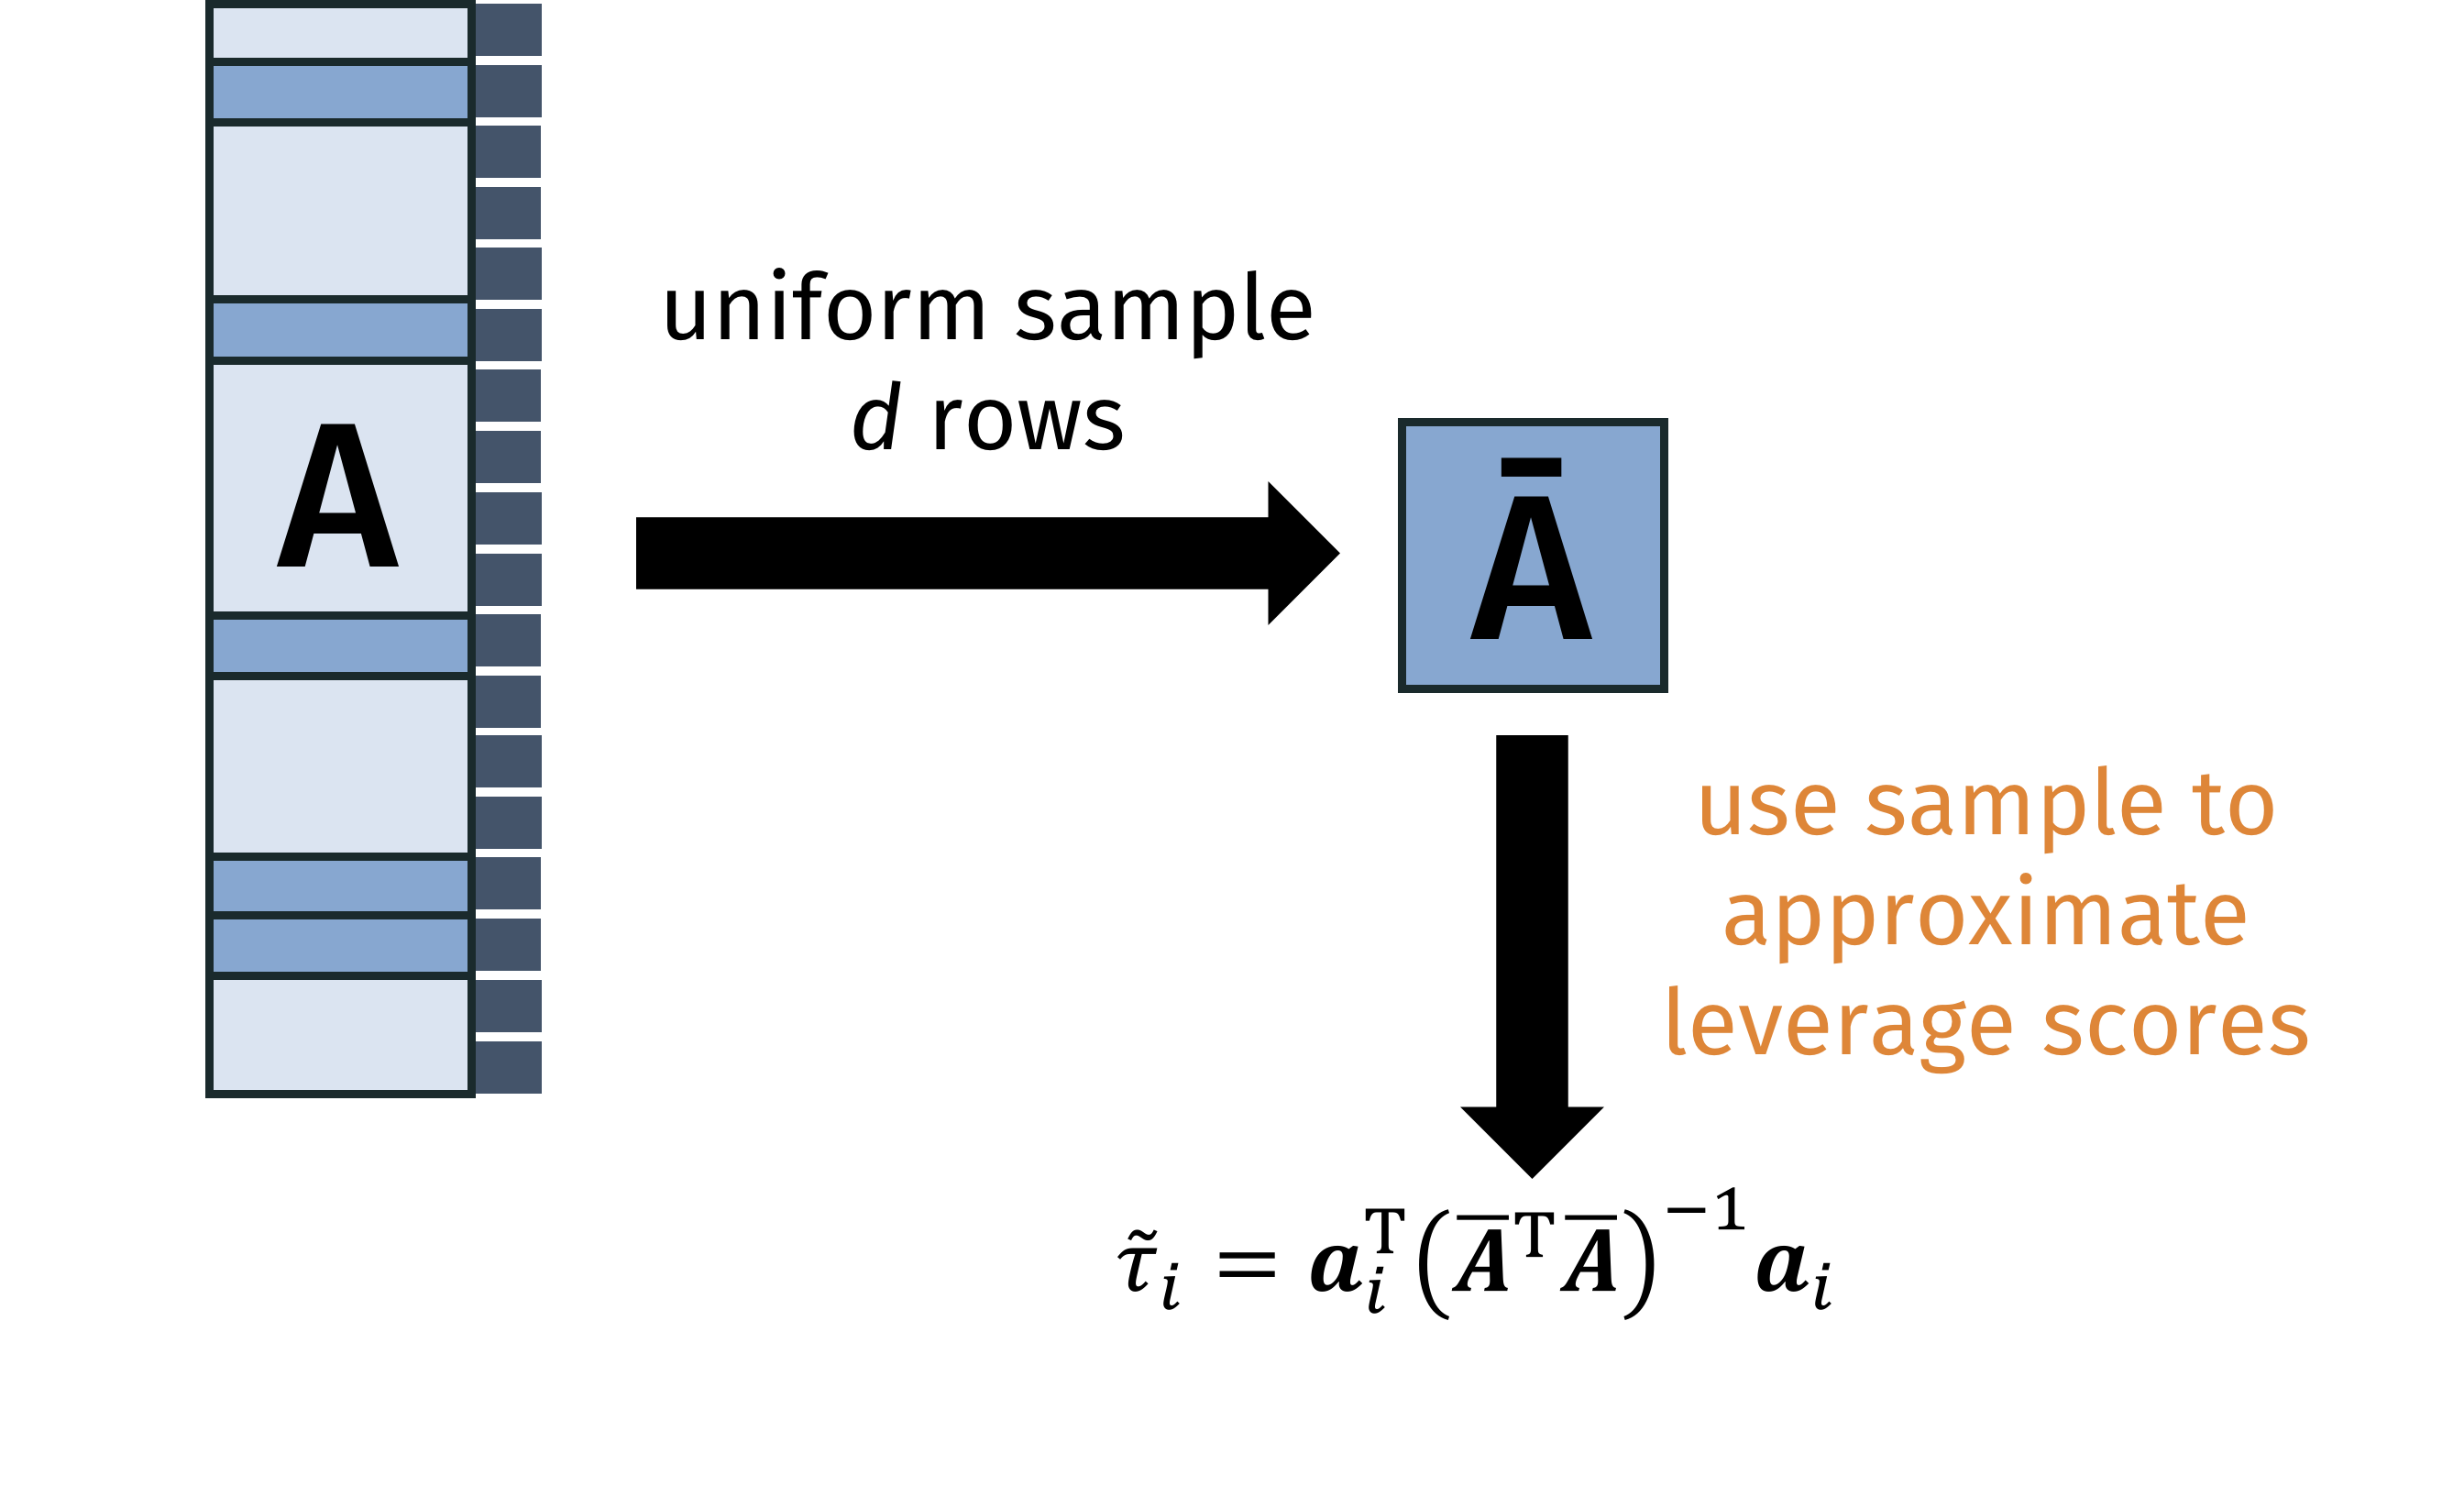
\includegraphics[width=.7\textwidth]{algo2.png}}
				\only<4>{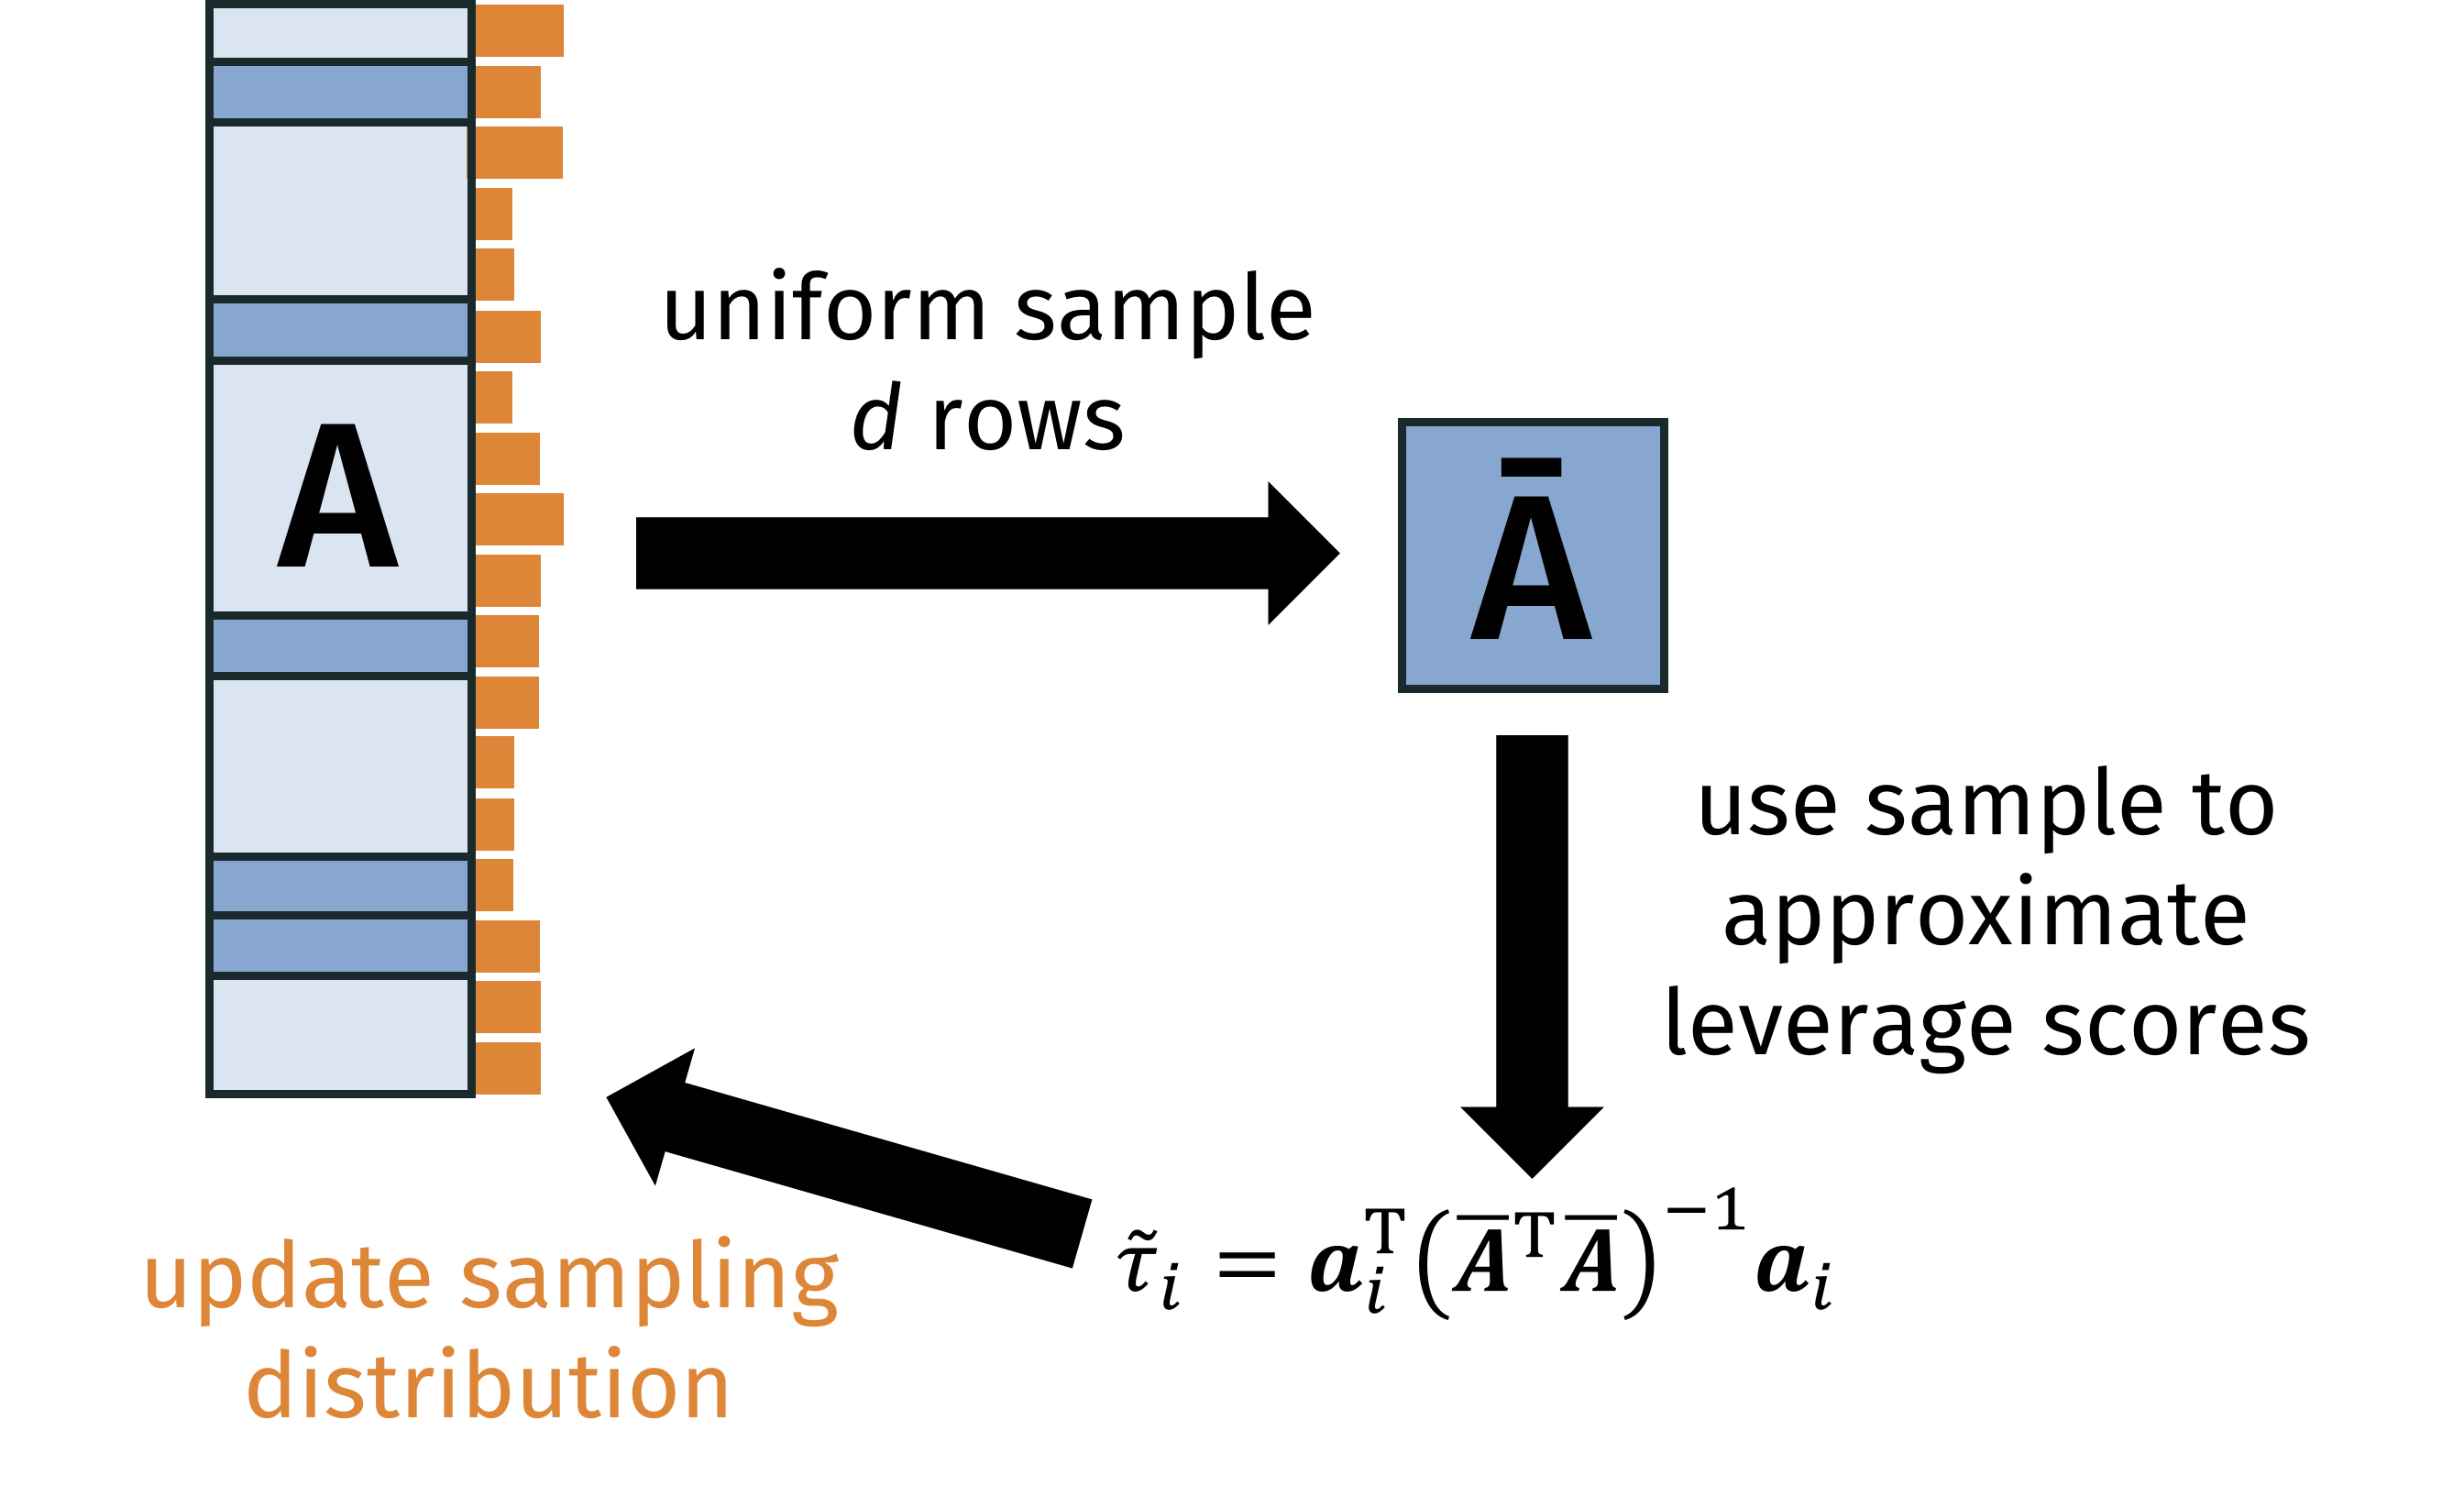
\includegraphics[width=.7\textwidth]{algo3.png}}
				\only<5>{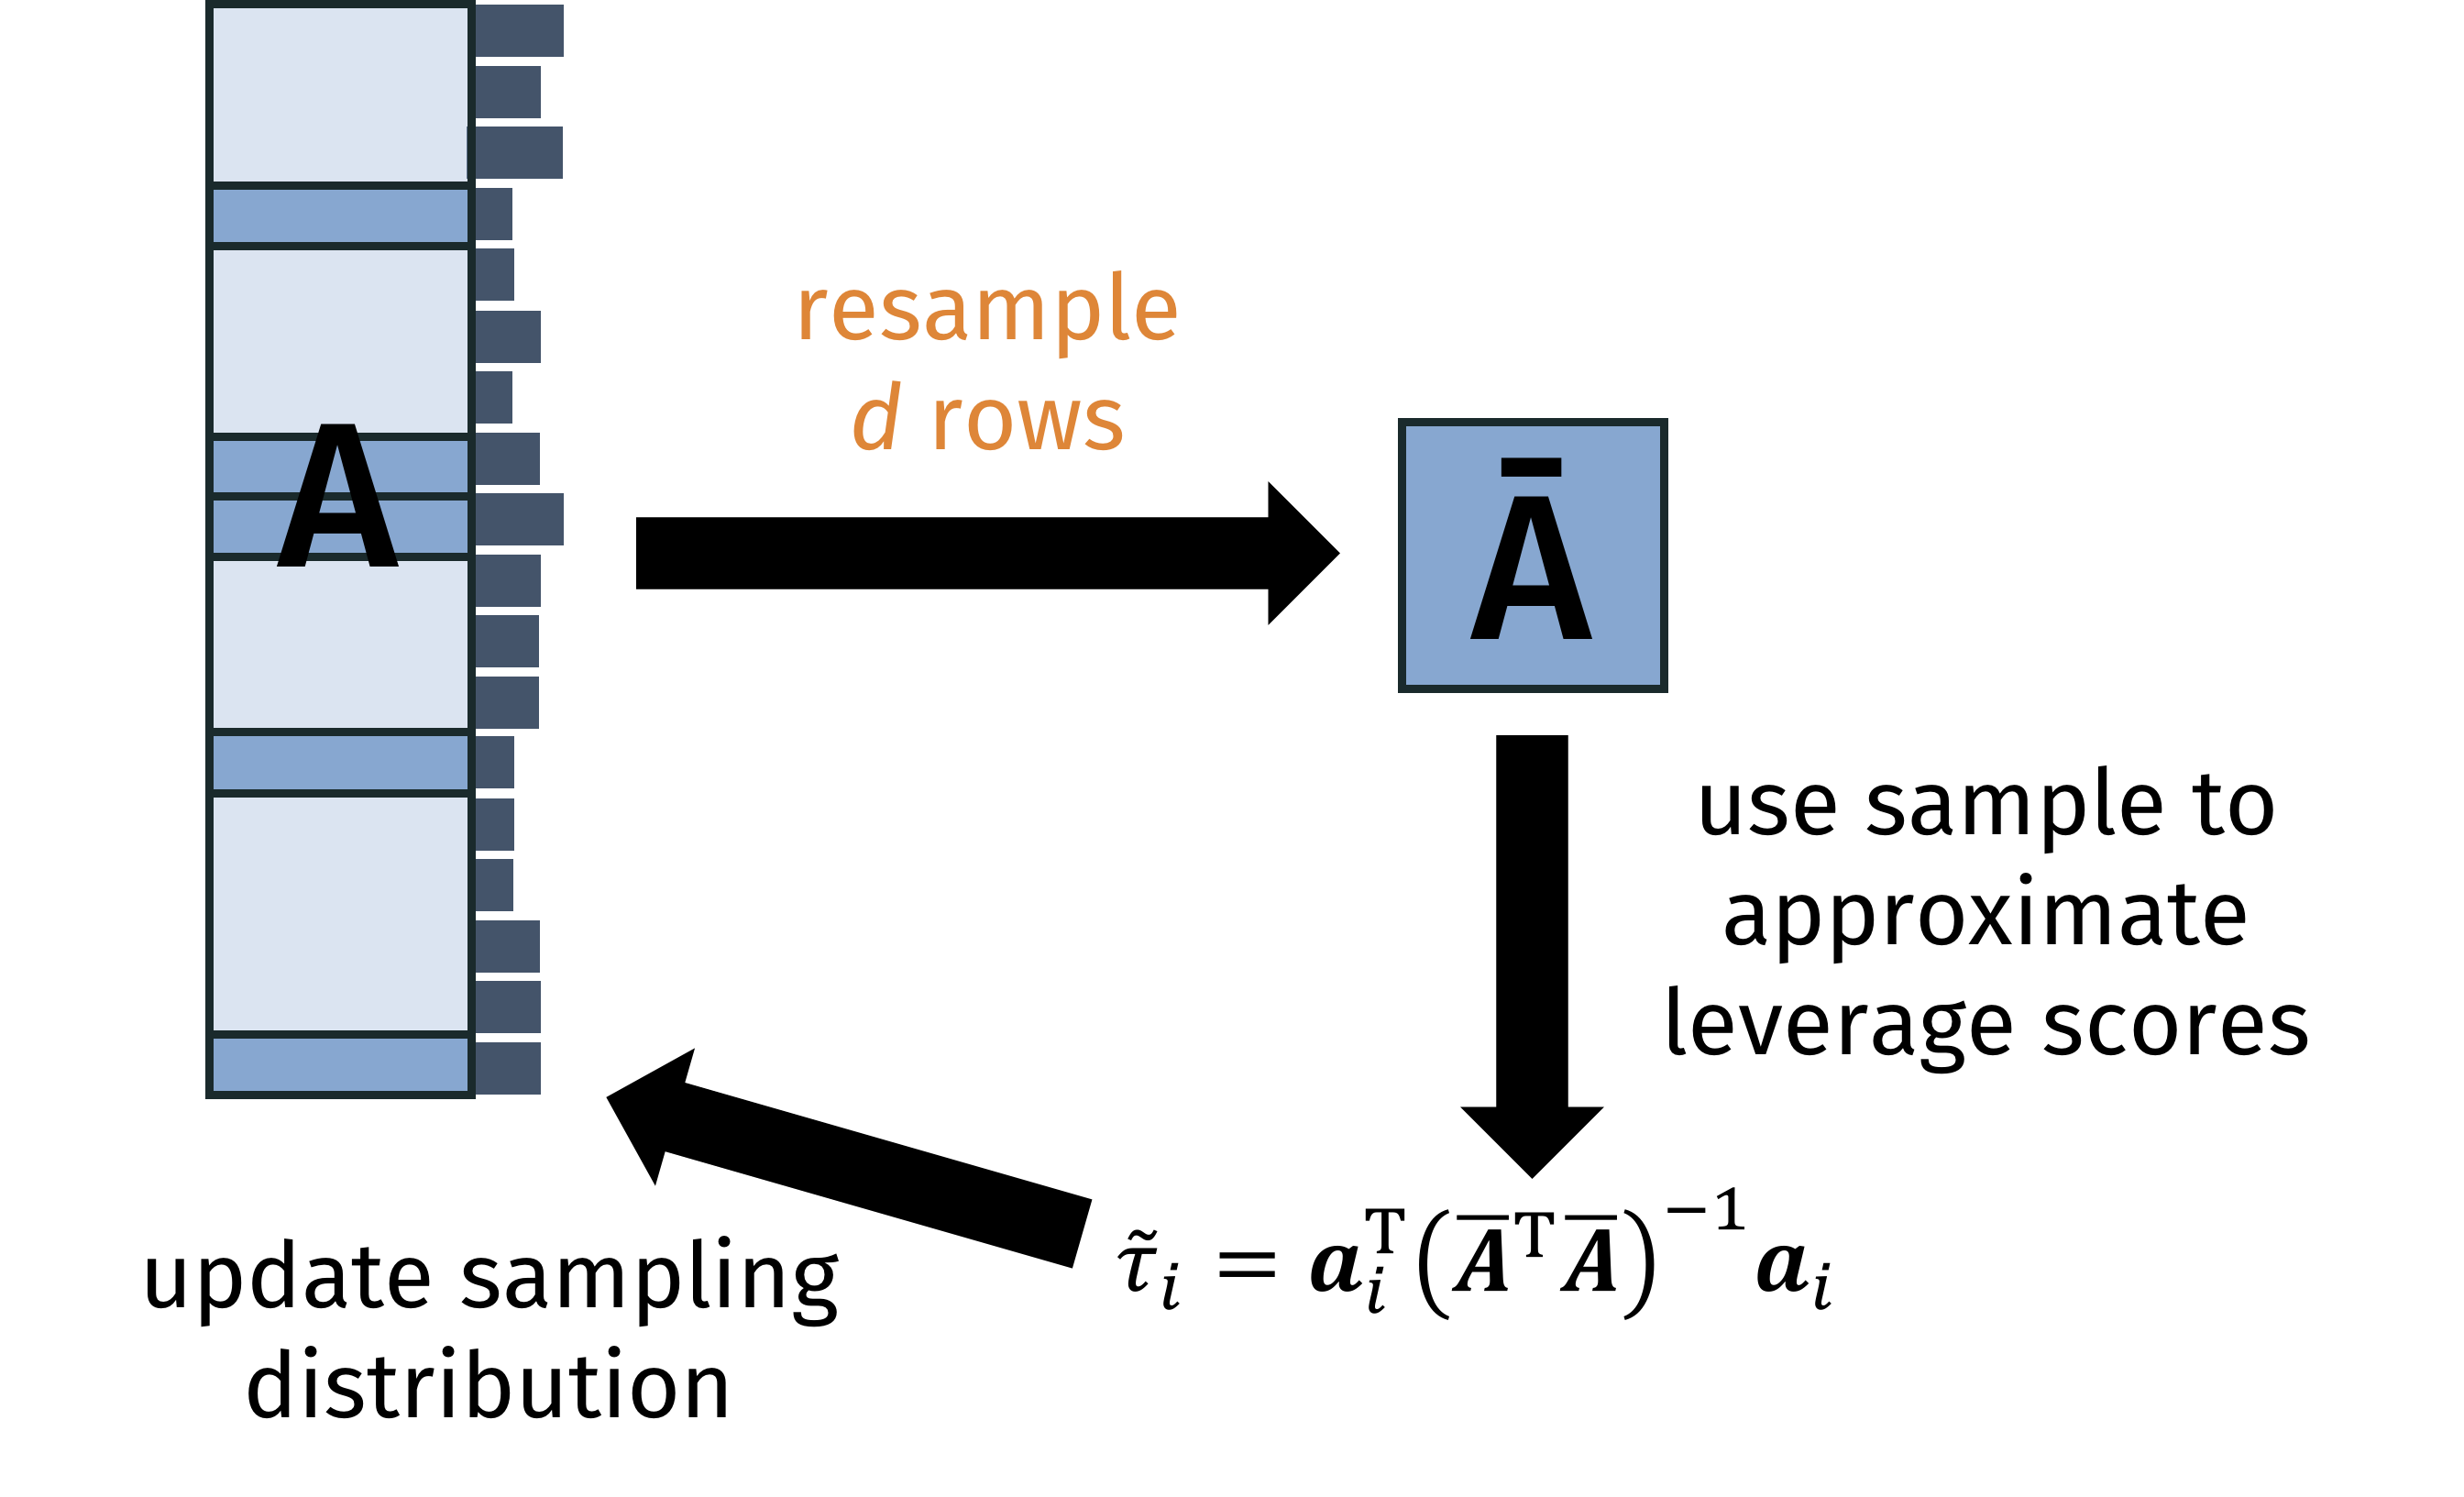
\includegraphics[width=.7\textwidth]{algo4.png}}
				\only<6>{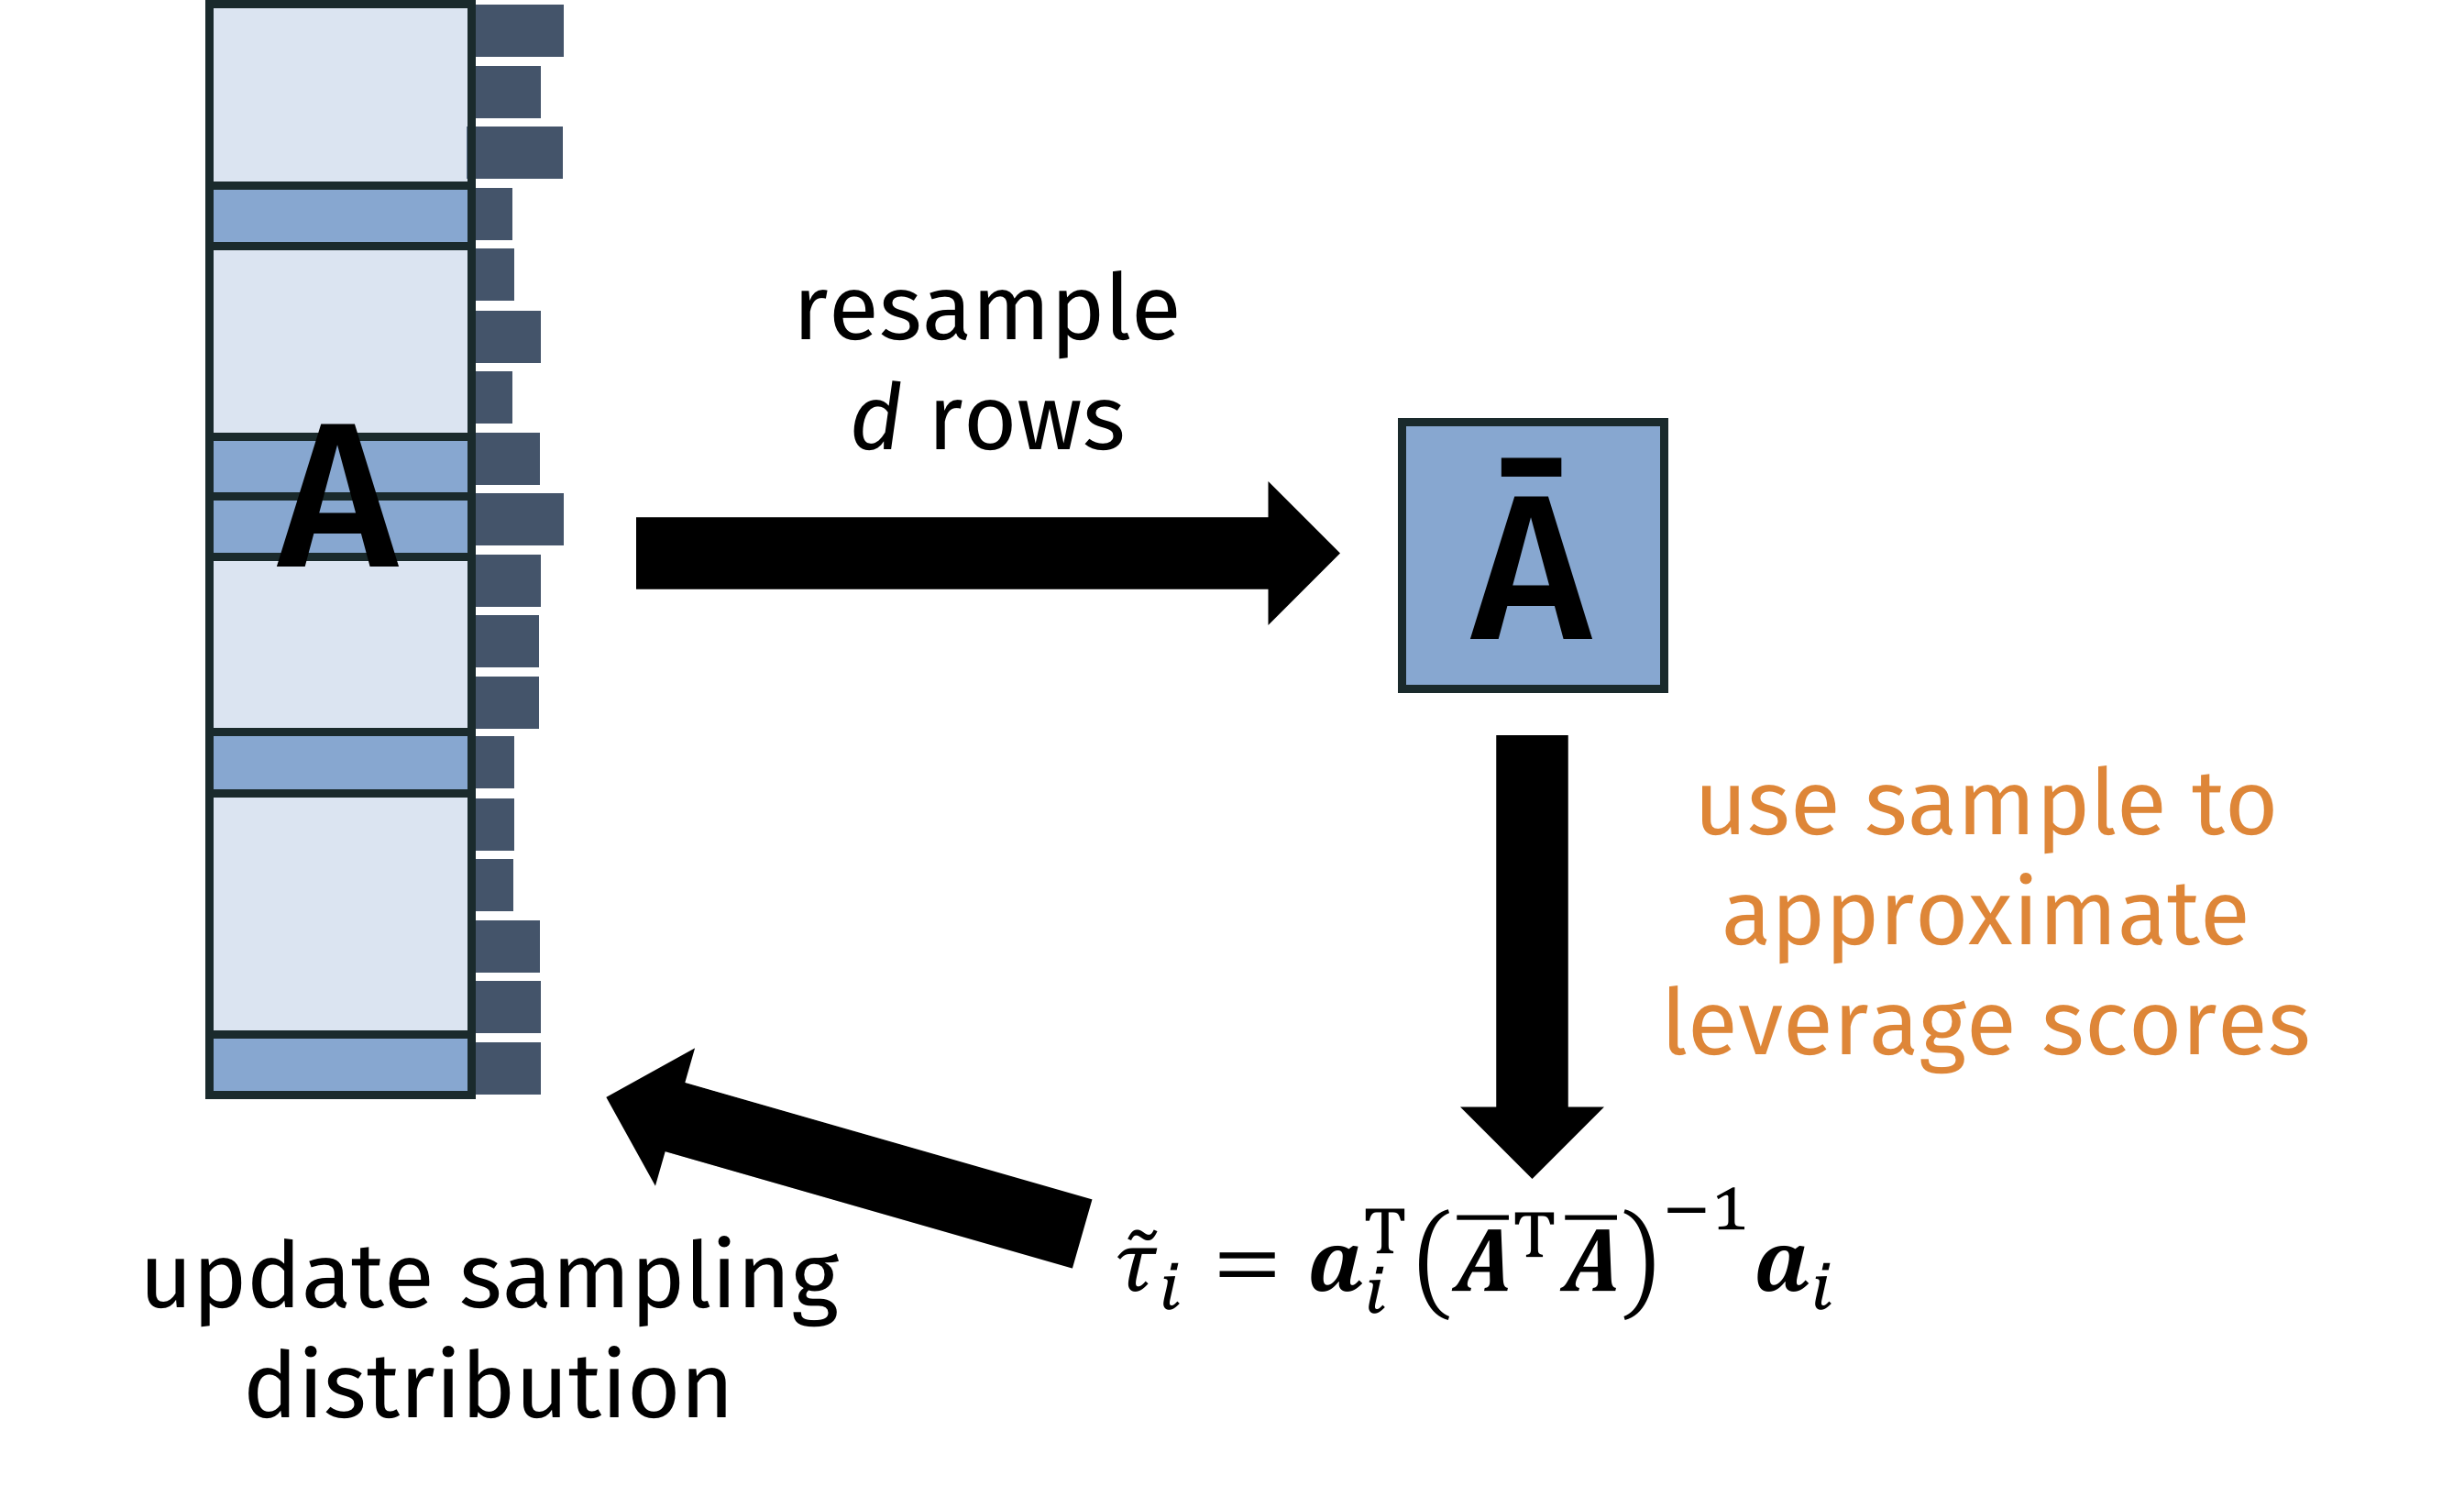
\includegraphics[width=.7\textwidth]{algo5.png}}
				\only<7->{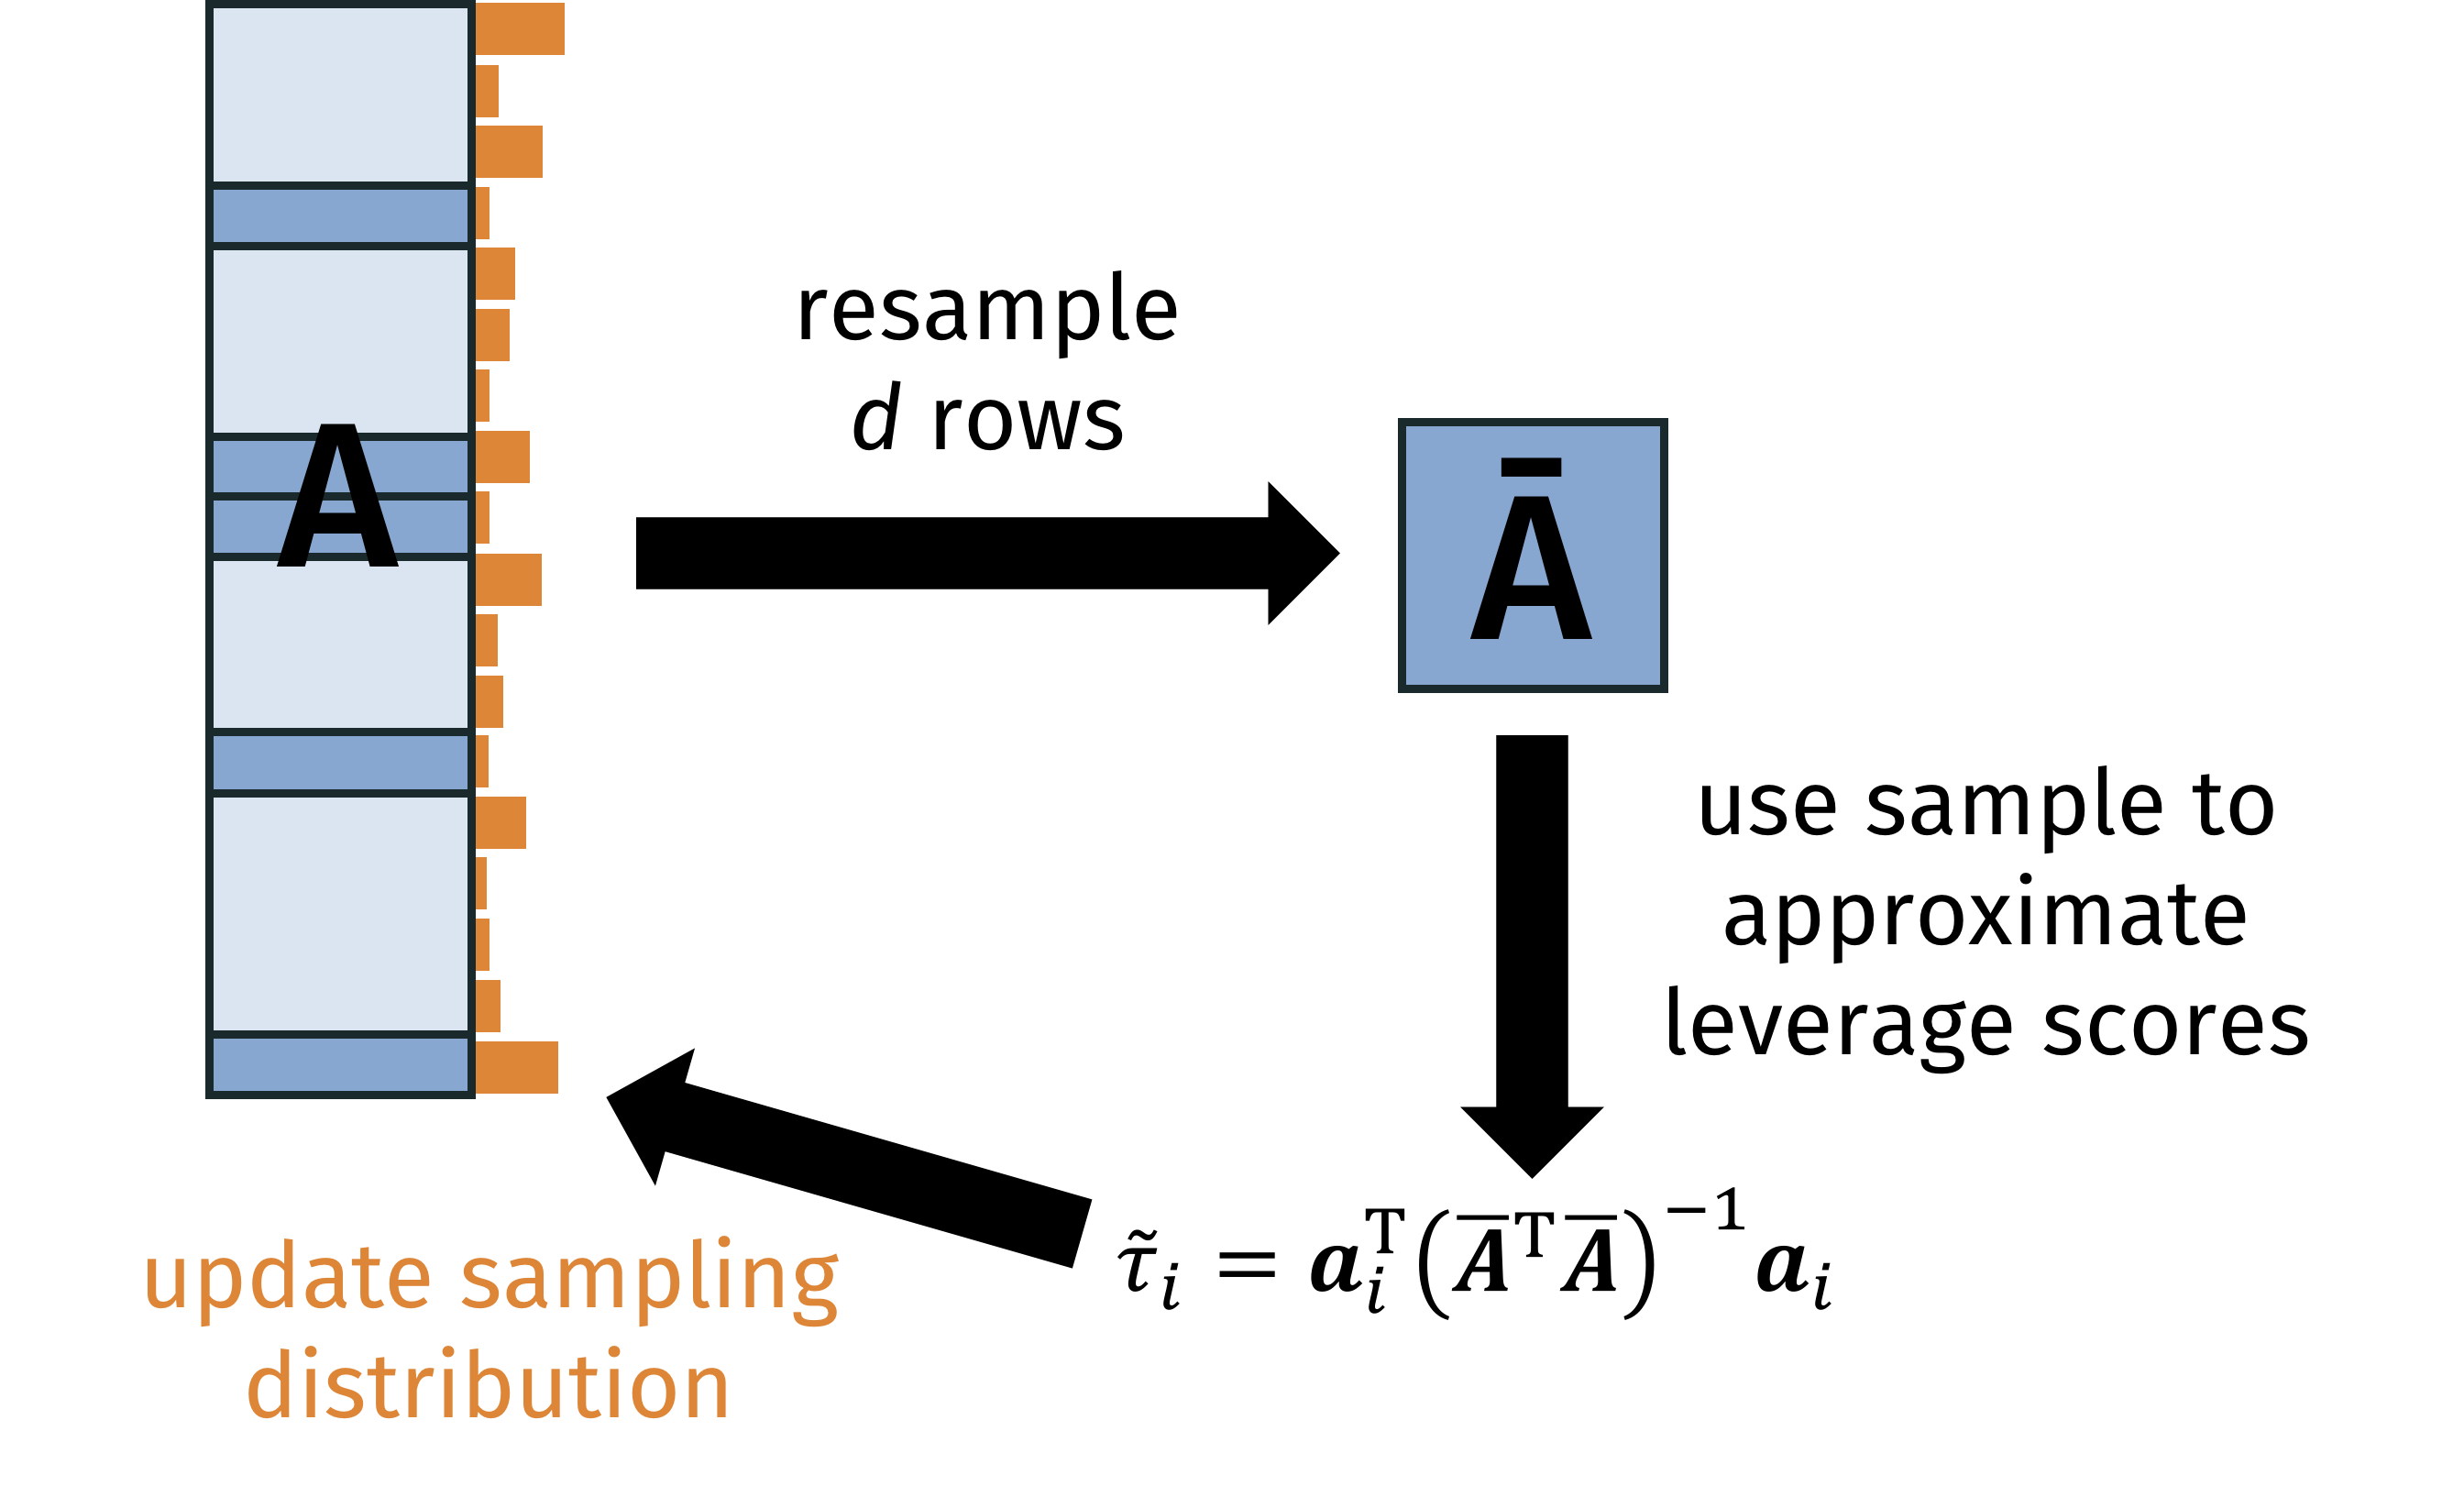
\includegraphics[width=.7\textwidth]{algo6.png}}}
			
			\uncover<8->{\vspace{-.5em} After $O(\log n)$ rounds, $\tilde{\tau_i} \approx \tau_i$ for all $i$.}
		\end{center}
		
	\vspace{-.5em}
			\textbf{Main algorithmic idea:} Bootstrap \emph{leverage score} sampling from \emph{uniform sampling} (ITCS 2015).
\end{frame}

\begin{frame}[t]
	\frametitle{some things i have worked on}
	\textbf{Problem}: Sometimes we want to compress down to $\ll d$ rows or columns. E.g. we don't need a full subspace embedding, but just want to find a near optimal rank $k$ approximation. 
	
	\textbf{Approach:} Use ``regularized'' version of the leverage scores:
	\begin{align*}
		\bar{\tau_i} = \bv{a}_i^T(\bv{A}^T\bv{A} + \lambda \bv{I})^{-1}\bv{a}_i
	\end{align*} 
	\begin{center}
		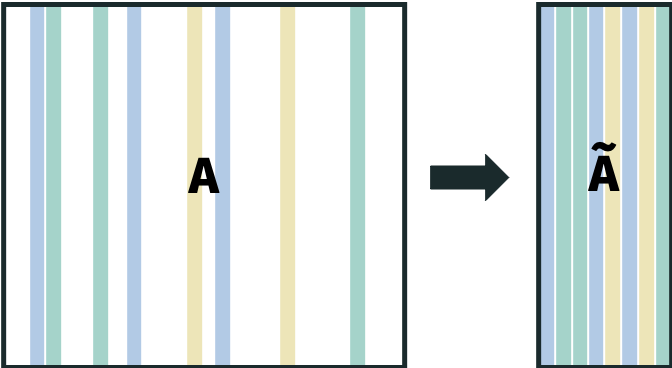
\includegraphics[width=.4\textwidth]{low_rank_compress.png}
	\end{center}
	\textbf{Result:} Sample $O(k\log k /\epsilon)$ columns whose span contains a near-optimal low-approximation to $\bv{A}$ (SODA 2017).
	
\end{frame}

\begin{frame}
	\frametitle{example result: sublinear time kernel approximation}
	The first $O(nk^2/\epsilon^2)$ time algorithm\footnote{NeurIPS 2017.} for near optimal rank-$k$ approximation of any $n\times n$ positive semidefinite kernel matrix:
	\begin{center}
		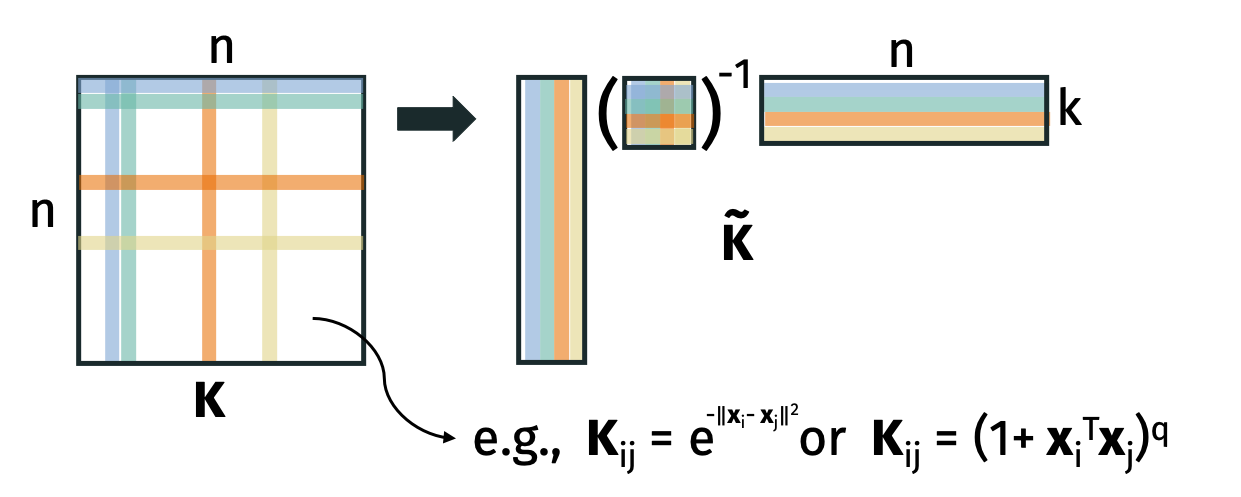
\includegraphics[width=.9\textwidth]{nystrom_approximation.png}
		
		Based on the classic Nystr\"{o}m method. Importantly, does not even require constructing $\bv{K}$ explicitly, which takes $O(n^2)$ time.
	\end{center}
\end{frame}


\end{document} 




